\documentclass[11pt,twoside]{report}
\usepackage{fancyhdr}                  % Fancy Header and Footer
\usepackage{threeparttable}
\usepackage{pdflscape}
\usepackage{longtable}
\usepackage{graphicx}
\usepackage{rotating}                  % Sideways of figures & tables
\usepackage[body={6.8in, 8.5in},left=1.25in,right=1.25in]{geometry}
%\usepackage[body={6.0in, 8.2in},left=1.25in,right=1.25in]{geometry}
                                       % Geometry package for easy page margin
                                       % setup
%\usepackage{amsmath,amssymb}           % AMS Math
%\usepackage[sectionbib]{natbib}        % Cross-reference package (Natural BiB)
%\usepackage{chapterbib}                % Put References at the end of each chapter
                                       % Do not put 'sectionbib' option here.
                                       % Sectionbib option in 'natbib' will do.
%\usepackage{setspace}                  % Line spacing
%\doublespacing
%\usepackage{txfonts}                   % Public Times New Roman text & math font
%
					% SOME USEFUL OPTIONS:
%%% Fancy Header %%%%%%%%%%%%%%%%%%%%%%%%%%%%%%%%%%%%%%%%%%%%%%%%%%%%%%%%%%%%%%%%%%
% Fancy Header Style Options
%\pagestyle{fancyplain}                       % Sets fancy header and footer
\pagestyle{fancy}                       % Sets fancy header and footer
\fancyhf{}                            % Delete current header and footer settings
\renewcommand{\chaptermark}[1]{         % Lower Case Chapter marker style
  \markboth{\chaptername\ \thechapter.\ #1}{}} %
\renewcommand{\sectionmark}[1]{         % Lower case Section marker style
  \markright{\thesection.\ #1}}         %
\fancyhead[RE]{\bfseries\leftmark}      % Chapter in the right on even pages
\fancyhead[LO]{\bfseries\rightmark}     % Section in the left on odd pages
\fancyfoot[LE,RO]{\bfseries\thepage}
\fancyfoot[LO,RE]{\bfseries GMI User's Guide}
\renewcommand{\headrulewidth}{0.4pt}    % Width of head rule
\renewcommand{\footrulewidth}{0.4pt}    % Width of foot rule
%
%\renewcommand{\plainheadrulewidth}{0.4pt}    % Width of head rule
%\renewcommand{\plainfootrulewidth}{0.4pt}    % Width of foot rule
%%%%%%%%%%%%%%%%%%%%%%%%%%%%%%%%%%%%%%%%%%%%%%%%%%%%%%%%%%%%%%%%%%%%%%%%%%%%%%%

%%%%%%%%%%%%%%%%%% END OF PREAMBULE %%%%%%%%%%%%%%%%%%
\begin{document}
\pagenumbering{roman}			% Roman numerals from abstract to text
\thispagestyle{empty}			% no page number on THIS page

\title{\Huge \bf Global Modeling Initiative: \\ Tutorial and User's Guide II}
\author{{\sc Jules Kouatchou, Megan Damon and Gary Wojcik} \\
{\Large\bf Software Integration and Visualization Office} \\
NASA Goddard Space Flight Center \\
Greenbelt, MD 20771}
%\date{ }
\maketitle

\newtheorem{remark}{Remark}
\newtheorem{example}{Example}
\newtheorem{definition}{Definition}
\newtheorem{conjecture}{Conjecture}
\newtheorem{theorem}{Theorem}
\newtheorem{Corollary}{Corollary}


%%%%%%%%%%%%%%%%%%%%%%%%%%%%%%%%%%%%%%%%%%%%%%%%%%%%%%%%%%%%%%%%%%%%%%%%%%%%%%%
%   Abstracts                                                                 %
%%%%%%%%%%%%%%%%%%%%%%%%%%%%%%%%%%%%%%%%%%%%%%%%%%%%%%%%%%%%%%%%%%%%%%%%%%%%%%%
\chapter*{Abstract\markboth{Abstract}{Abstract}}
% Mark 'Abstract' both even and odd markers

In this report, we provide a description of the GMI code.
It is intended to help users in the GMI community
to obtain, install, compile, run, and modify the code.
We present the code organization and data structures,
procedures on how to run the code under various configurations,
to manipulate the code, and the code parallel
performance.  
Examples introduced here were carried out on Intel clusters.

\vskip 0.5cm

\noindent
This version of the User's Guide differs from the previous one
(released in 2004) in many areas due to the fact that the GMI
code went through a lot of changes. For instance:
%
\begin{itemize}
\item A completely new code directory structure
\item Componentization of the code
\item New resource file settings
\item New diagnostics capabilities.
\item Removal of the LLNL ESM package
\item Introduction of ESMF.
\end{itemize}
%
As a result of these changes, we have new installation and compilation
procedures, an object-oriented approach to manipulate components of
the code, a more flexible way to produce netCDF output file, a more
readable code, the ability to automatically generate code documentation, 
etc.

%%%%%%%%%%%%%%%%%%%%%%%%%%%%%%%%%%%%%%%%%%%%%%%%%%%%%%%%%%%%%%%%%%%%%%%%%%%%%%%%
%   Acknowledgements                                                          %
%%%%%%%%%%%%%%%%%%%%%%%%%%%%%%%%%%%%%%%%%%%%%%%%%%%%%%%%%%%%%%%%%%%%%%%%%%%%%%%
\chapter*{Acknowledgements\markboth{Acknowledgements}{Acknowledgements}}


\tableofcontents
\listoftables
\listoffigures

%\newpage


\pagenumbering{arabic}			% Arabic page numbers from now on
%
\chapter[Introduction]{Introduction} \label{chap:introduction}
%\section{Overview of the Model}
%\pagenumbering{arabic}			% Arabic page numbers from now on
%
The Global Modeling Initiative (GMI) 
\footnote{http://gmi.gsfc.nasa.gov/gmi.html}
was initiated under the auspices of the Atmospheric Effects of Aircraft 
Program (AEAP) in 1995. 
The goal of GMI is to develop and maintain a state-of-the-art
modular 3-D chemistry transport model (CTM) that can be used
to assess the impact of various natural and anthropogenic
perturbations on atmospheric composition and chemistry, including,
but not exclusively, the effect of aircraft.

The Atmospheric Chemistry Modeling and Analysis Program (ACMAP)
 has selected the approach of GMI to serve
both as an assessment facility and a testbed for model improvements
for future assessment in all areas of atmospheric chemistry.
%
The goals in the design of GMI as an assessment tool are \cite{Kinnison-etal01}
%
\begin{enumerate}
\item The model should be well-characterized and thoroughly tested
      against observations.
\item The model should be able to test and compare a diversity of
      approaches to specific processes by being able to easily swap
      modules containing different formulations of chemical
      processes, within a common framework.
\item The model should be optimized for computational efficiency and
      be able to run on different platforms.
\item Model results should be examined by a large representation of
      the scientific community, thus faciliting consensus on the significance
      of assessment results.
\item Ultimately, the model integration could provide a unique assessment
      capability for other anthropogenic impacts of concern by providing
      a testbed for other algorithms and intercomparisons used in
      assessment of those issues.
\end{enumerate}
%
Many elements of the GMI model address these goals.
The GMI model is a modular chemistry-transport model (CTM) with
the ability to carry out multi-year assessment simulations as
well as incorporate different modules, such as meteorological
fields, chemical mechanisms, numerical methods, and other modules
representing the different approaches of current models. This
capability facilitates the understanding of the differences
and uncertainties of model results.

The testing of GMI results against observations is a high priority
of GMI activities. Science Team members contribute by either
supplying a particular module and/or contributing to the analysis
of the results and comparison with atmospheric observations
\cite{Douglass-etal99, Rotman-etal01, Strahan-Duncan-Hoor07, Meskhidze-etal07}. 
Application of the model to the potential impacts of
stratospheric aircraft emissions is presented in \cite{Kinnison-etal01}. 
The model has been employed to investigate the effects of stratospheric aircraft
emissions on polar stratospheric clouds \cite{Considine-etal00} and simulate
ozone recovery over a 36-year time period \cite{Considine-etal04}.

Besides acting as a testbed for different modules, GMI will also
act as a 3-D assessment facility. The GMI modular code is currently
implemented at NASA/Goddard Space Flight Center (the core institution).
The core institution is responsible for: 
%
\begin{itemize}
\item Integrating and testing components of the GMI model, 
\item Making the code readable, flexible and easy to maintain
\item Maintaining coding standards which will make the model 
      portable to different platforms
\item Carrying out assessment calculations, and 
\item Providing first-order results and diagnostics for 
      analysis by team members. 
\end{itemize}
%
The current  version of the code has been developed to run on a variety of 
computing platforms, both with single and multiple processors 
(Linux clusters, SGI Origin series, HP Compaq SC45, 
single processor workstations, etc.).

This report is intended to familiarize users with the GMI code.
Users will be able to 
\begin{itemize}
\item Have information on the code structure (Chapter \ref{chap:structure}).
\item Obtain instructions on how to obtain the code, install it, 
      compile it, run it on any platform (Chapter \ref{chap:installation}).
\item Have knowledge of all the input and output files involved in the
      code (Chapter \ref{chap:files}, Appendix \ref{chap:netcdf} and
      Appendix \ref{chap:rcFile}).
\item Carry out specific and restart runs (Chapter \ref{chap:runs}).
\item Learn how to make changes in the code (Chapter \ref{chap:changes}).
\item Execute useful script tools needed, for instance, to search
      for words, to produce restart input resource files, etc.
      (Chapter \ref{chap:script}).
\item Learn basic CVS commands (Chapter \ref{chap:cvs}).
\item Analyze the parallel performance of the code 
      (Chapter \ref{chap:performance}).
\item Be familiar with include files used to select the desired architecture,
      to set up compilation options, etc. (Appendix \ref{chap:inc_files}).
\item Know how to carry out a single or multiple processor run 
      (Appendix \ref{chap:proc_runs}).
\item Use resource file features (Appendix \ref{chap:features}).
\item Know the species used in the code (Appendix \ref{chap:listSpecies}).
\end{itemize}

\chapter[Structure of the Code]{Structure of the Code}
\label{chap:structure}
%
%
%
\section{Components of GMI}
%
The modules that make up the GMI assessment model are \cite{Rotman-etal01}:
%
\begin{enumerate}
\item Input meteorological data coming from four major Global Circulation
      Models (from NCAR, GISS, DAO, and GMAO). Data from all these input
      sets include horizontal U and V winds, temperature, and surface
      pressure.
\item Advection algorithm to transport trace species
\item Mass tendencies
\item Numerical schemes for chemistry solutions
\item Chemistry mechanism
\item Heterogeneous processes
\item Photolysis
\item Diagnostics
\item Tropospheric treatment
\item Initial conditions
\item Boundary conditions
\end{enumerate}
%
All the above modules have multiple packages/versions that can be selected through
proper resource file settings.
The GMI model incorporates six chemical mechanisms:
\begin{itemize}
\item aerosol (University of Michigan formulation)
\item micro\_aerosol (University of Michigan formulation)
\item gocart\_aerosol (GOCART formulation)
\item stratosphere
\item troposphere
\item combined stratostophere/troposphere (strat\_trop or combo)
\end{itemize}
%
A summary of the mechanisms appears in Table \ref{tab:mecha}.
%

{\small
\begin{center}
\begin{table}[!h]
\begin{tabular}{|l|c|c|c|} \hline\hline
Mechanism name      & $\#$ species & $\#$ thermal reactions & $\#$ photolytic reactions  \\ \hline\hline
aerosol         & 30  &  8  &  1  \\
micro\_aerosol  & 40  &  8  &  1  \\
gocart\_aerosol & 31  &  8  &  1  \\
stratosphere    & 57  & 122 & 44  \\
troposphere     & 85  & 222 & 49  \\
strat\_trop     & 124 & 320 & 81  \\ \hline\hline
\end{tabular}
\caption{Basic information on the chemical mechanisms.}
\label{tab:mecha}
\end{table}
\end{center}
}

%
\section{Directory Structure of The Code}
%
The top directory of the GMI code is {\em gmi\_gsfc/}
which contains the sub-directories 
%
\begin{itemize}
\item {\em Components/}: Routines for each component
\item {\em Shared/}: Include files and routines shared by all the components
\item {\em Documents/}: General information about the code and how it is to be used
\item {\em Applications/}: Routines for driving the code
\item {\em Config/}: Main makefile files
\end{itemize}
%
In Table \ref{ta:gmi_dir4}, 
we give more details on the structure of each of the above directories.

{\small

\begin{landscape}

\begin{center}
\begin{longtable}{|l|l|} \hline \hline
{\bf Directory Name}                & {\bf Synopsis} \\ \hline\hline
{\bf gmi\_gsfc }                          & GMI reference directory \\ \hline
gmi\_gsfc/Documents                       & Directory for documents                 \\ \hline
gmi\_gsfc/Documents/Papers                &                                       \\ \hline
gmi\_gsfc/Documents/Tutorials             &                         \\ \hline
gmi\_gsfc/Documents/Tutorials/UserGuide   & This document           \\ \hline
gmi\_gsfc/Documents/Tutorials/removingESM   &                         \\ \hline
gmi\_gsfc/Documents/Tutorials/MEGANemissions &                         \\ \hline
gmi\_gsfc/Documents/ReadmeFiles           &                                       \\ \hline
gmi\_gsfc/Config                          &  Main makefile files \\  \hline
gmi\_gsfc/Shared               & Files and modules shared by all the components \\ \hline
gmi\_gsfc/Shared/GmiCommunications        &  Communication routines             \\ \hline
gmi\_gsfc/Shared/GmiIOutilities         &   Supporting routines for I/O          \\ \hline
gmi\_gsfc/Shared/GmiESMF                &  Interfaces to ESMF                      \\ \hline
gmi\_gsfc/Shared/GmiInclude         &   Include files                              \\ \hline
gmi\_gsfc/Shared/GmiMetFields         &  Routines for deriving MetFields variables   \\ \hline
gmi\_gsfc/Shared/GmiScripts         &   Script tools                                   \\ \hline
gmi\_gsfc/Shared/GmiSupportingModules & Supporting routines for various calculations.  \\ \hline
gmi\_gsfc/Shared/NcUtils\_Double         & netCDF utility routines for double precision \\ \hline
gmi\_gsfc/Shared/NcUtils\_Single         & netCDF utility routines for single precision  \\ \hline
gmi\_gsfc/Components/GmiAdvection        & Advection component \\ \hline
gmi\_gsfc/Components/GmiAdvection/advectionMethod & Routines driving Advection \\ \hline
gmi\_gsfc/Components/GmiAdvection/dao2advec       & DAO advection routines \\ \hline
gmi\_gsfc/Components/GmiAdvection/dao2utils       & Advection utility routine computing, \\
                                             & courant numbers, Divergence, etc. \\ \hline
gmi\_gsfc/Components/GmiAdvection/include     & Advection include file \\ \hline
gmi\_gsfc/Components/GmiChemistry             & Chemistry component  \\ \hline
gmi\_gsfc/Components/GmiChemistry/chemistryMethod  & Routines driving Chemistry \\ \hline
gmi\_gsfc/Components/GmiChemistry/AerosolDust  &  Module for Aerosol/Dust calculations \\ \hline
gmi\_gsfc/Components/GmiChemistry/ioChemistry  &  I/O routines for Chemistry \\ \hline
gmi\_gsfc/Components/GmiChemistry/include     & Chemistry include file \\ \hline
gmi\_gsfc/Components/GmiChemistry/sad  & Aerosol surface area density and condensed   \\
                                             & phase mixing ratio modules \\ \hline
gmi\_gsfc/Components/GmiChemistry/solvers  &  Chemistry solvers \\ \hline
gmi\_gsfc/Components/GmiChemistry/solvers/micro\_sulfur  &  \\ \hline
gmi\_gsfc/Components/GmiChemistry/solvers/smv2chem  &  \\ \hline
gmi\_gsfc/Components/GmiChemistry/solvers/sulfur  &  \\ \hline
gmi\_gsfc/Components/GmiChemistry/mechanisms    & Chemical mechanisms \\ \hline
gmi\_gsfc/Components/GmiChemistry/mechanisms/aerosol                     & Aerosol chemistry \\ \hline
gmi\_gsfc/Components/GmiChemistry/mechanisms/aerosol/include\_setkin     & Include files for aerosol \\ \hline
gmi\_gsfc/Components/GmiChemistry/mechanisms/aerosol/setkin              & Routines for rate constants and kinetic rates \\ \hline
gmi\_gsfc/Components/GmiChemistry/mechanisms/micro\_aerosol  & micro\_aerosol chemistry \\ \hline
gmi\_gsfc/Components/GmiChemistry/mechanisms/micro\_aerosol/include\_setkin     & Include files for micro\_aerosol \\ \hline
gmi\_gsfc/Components/GmiChemistry/mechanisms/micro\_aerosol/setkin              & Routines for rate constants and kinetic rates \\ \hline
gmi\_gsfc/Components/GmiChemistry/mechanisms/gocart\_aerosol & gocart\_aerosol chemistry \\ \hline
gmi\_gsfc/Components/GmiChemistry/mechanisms/gocart\_aerosol/include\_setkin & Include files for gocart\_aerosol \\ \hline
gmi\_gsfc/Components/GmiChemistry/mechanisms/gocart\_aerosol/setkin          & Routines for rate constants and kinetic rates \\ \hline
gmi\_gsfc/Components/GmiChemistry/mechanisms/strat\_trop                 & Strat/Trop chemistry \\ \hline
gmi\_gsfc/Components/GmiChemistry/mechanisms/strat\_trop/include\_setkin & Include files for the combined strat/trop \\ \hline
gmi\_gsfc/Components/GmiChemistry/mechanisms/strat\_trop/setkin          & Routines for rate constants and kinetic rates \\ \hline
gmi\_gsfc/Components/GmiChemistry/mechanisms/stratosphere                & Stratospheric chemistry \\ \hline
gmi\_gsfc/Components/GmiChemistry/mechanisms/stratosphere/include\_setkin& Include files for stratosphere \\ \hline
gmi\_gsfc/Components/GmiChemistry/mechanisms/stratosphere/setkin         & Routines for rate constants and kinetic rates \\ \hline
gmi\_gsfc/Components/GmiChemistry/sulfur                      & Routines for sulfur chemistry \\ \hline
gmi\_gsfc/Components/GmiChemistry/mechanisms/troposphere      & Tropospheric chemistry \\ \hline
gmi\_gsfc/Components/GmiChemistry/mechanisms/troposphere/include\_setkin & Include files for troposphere \\ \hline
gmi\_gsfc/Components/GmiChemistry/mechanisms/troposphere/setkin          & Routines for rate constants and kinetic rates \\ \hline
gmi\_gsfc/Components/GmiChemistry/photolysis & Photolysis component \\ \hline
gmi\_gsfc/Components/GmiChemistry/photolysis/include & \\ \hline
gmi\_gsfc/Components/GmiChemistry/photolysis/fastj & \\ \hline
gmi\_gsfc/Components/GmiChemistry/photolysis/fast\_JX & \\ \hline
gmi\_gsfc/Components/GmiChemistry/photolysis/fast\_JX53b & \\ \hline
gmi\_gsfc/Components/GmiChemistry/photolysis/fast\_JX53c\_ref & \\ \hline
gmi\_gsfc/Components/GmiChemistry/photolysis/lookup & Routines for lookup table \\ \hline
gmi\_gsfc/Components/GmiChemistry/photolysis/utils & \\ \hline
gmi\_gsfc/Components/GmiConvection & Convection component \\ \hline
gmi\_gsfc/Components/GmiConvection/convectionMethod & Routines driving Convection \\ \hline
gmi\_gsfc/Components/GmiDeposition & Deposition component \\ \hline
gmi\_gsfc/Components/GmiDeposition/depositionMethod &  Routines driving Deposition  \\ \hline
gmi\_gsfc/Components/GmiDeposition/include &                     \\ \hline
gmi\_gsfc/Components/GmiDiffusion         & Diffusion component \\ \hline
gmi\_gsfc/Components/GmiDiffusion/diffusionMethod  & Routines driving Diffusion \\ \hline
 gmi\_gsfc/Components/GmiEmission  & Emission component \\ \hline
gmi\_gsfc/Components/GmiEmission/emissionMethod  & Routines driving Emission \\ \hline
gmi\_gsfc/Components/GmiEmission/Harvard & Harvard emission routines \\ \hline
gmi\_gsfc/Components/GmiEmission/MEGAN & MEGAN emission routines \\ \hline
gmi\_gsfc/Components/GmiEmission/ioEmission & I/O routines for Emission \\  \hline
gmi\_gsfc/Components/GmiEmission/include &  \\ \hline
gmi\_gsfc/Components/GmiEmission/lightning & Routines for lightning parameterization  \\ \hline
gmi\_gsfc/Components/GmiEmission/llnl & LLNL emission routines \\ \hline
gmi\_gsfc/Components/GmiSpeciesConcentration & Species Concentration component \\ \hline
gmi\_gsfc/Components/GmiSpeciesConcentration/spcConcentrationMethod & Routines driving Species Concentration\\ \hline
gmi\_gsfc/Components/GmiSpeciesConcentration/ioSpcConcentration & I/O routines for Species Concentration \\ \hline
gmi\_gsfc/Applications & Control and time stepping routines \\ \hline
gmi\_gsfc/Applications/GmiApp &  \\ \hline
gmi\_gsfc/Applications/GmiBin &  \\ \hline\hline
\caption{GMI code directories}
\label{ta:gmi_dir4}
\end{longtable}
\end{center}

\end{landscape}

}

\section{Coding Principles}
%
A ".F90" (Fortran code) suffix denotes source code files.
The "F90" suffix indicates that the Fortran source contains
preprocessing directives.
Files named with a ".h" suffix are header files that contain
preprocessing directives, variable declarations, parameter definitions,
and common block definitions.
Contents of selected header files are included via $\# include$ statements
at the beginning portion of each of the ".F90" and ".c" files.

To enable multiyear chemistry simulations, the GMI core model was
parallelized to make use of the most powerful computational
platforms available.
The parallel strategy uses a two-dimensional longitude/latitude
domain decomposition whereby each subdomain consists of a number
of contiguous columns having a full vertical extent.
Processors are assigned to subdomains, and variables local to a given
subdomain are stored on the memory of the assigned processor.
Data are transmitted between computational processes, when needed,
in the form of messages.
The number of meshpoints per subdomain may not be uniform, under the
constraint that the decomposition be logically rectangular.
The choice to decompose in only two dimensions is based on the
fact that chemistry, photolysis, and cold sulfate algorithms make
up the vast majority of the computational requirements and are
all either local or column calculations.
These computations require no communication with neighboring grid
zones and hence maximize the parallel efficiency
\cite{Rotman-etal01}.
 
\section{General Flowchart of the Code}
%
In this section, we provide flowcharts of the main program and the time stepping
routine. 
The main program is {\em gmiMain} (filename gmiMain.F90).
This calls routines to initialize the ESMF programming environment
(that launches the Message Passing Interface MPI),  perform domain decomposition, 
initialize the GMI
components (Chemistry, Emission, Deposition, Advection, Convection, and Diffusion),
perfom model integration (run the components), and finalize the components
and ESMF (see Figure \ref{fig:main}).
%
%
%
\begin{figure}[hbtp]
\centering                                             % center the figure
\includegraphics[height=6.0in,width=6.0in]{gmiMainFlowchart.ps}
\caption{Flowchart of the main program} 
\label{fig:main}
\end{figure}
%
The most important calculations done in the time stepping routine appear in
Figure \ref{fig:step}.
The figure only shows the main modules of the code.
We observe that the major components are executed here.
%
\begin{figure}[hbtp]
\centering                                             % center the figure
\includegraphics[height=7.95in,width=6.50in]{gmiSteppingFlowchart.ps}
\caption{Flowchart of the time stepping routine.}
\label{fig:step}
\end{figure}


%
\chapter[Installation and Testing]{Installation and Testing}
\label{chap:installation}
%
This chapter is written to help new users install and 
test the GMI code. 
We provide specific instructions on how to obtain the code, 
to properly set environment variables, to select the model 
configuration, to choose a particular platform, 
to compile the code and to perform basic test runs. 
The focus of these instruction is on the installation and execution of 
the GMI code on {\tt discover} and {\tt explore}. 
The same procedures can easily be applied to any platform.

To get and install the GMI code, the following system software is needed:
%
\begin{itemize}
\item CVS (see Chapter \ref{chap:cvs} for instruction)
\item F90/95 (ideally {\em ifort} for intel)
\item C (ideally {\em icc} for intel). Down the road, it will not be required.
\item MPI 
\item netCDF (version 3.4 or higher). The location of netCDF should be
      provided in the files {\em Config/gem\_config.h} and {\em Config/compiler.mk}
      before compiling the code (see Section \ref{sec:envi} for details).
\item ESMF (see {\tt http://www.esmf.ucar.edu}) 
\item make and gmake
\item makedepend (generally in /usr/bin/X11)
\item perl
\item a debugger (if possible)
\end{itemize}


%
%\section{Installation and Testing}
During this process of installing and testing the code, it is 
assumed that {\em Cshell} is the default shell employed by the user.
In fact, the GMI environment variables required for these procedures are
set up using {\em Cshell}.

\section{Getting the Code}
%
To obtain the GMI code,
%
\begin{itemize}
\item Select the directory where you want to install the GMI model, 
      say {\em MYGMI/}
\item Get the latest version of the model from the cvs repository at 
      {\em sourcemotel} by typing the command lines:
\end{itemize}
%
\begin{verbatim}
        %setenv CVS_RSH ssh
        %cvs -d usrid@sourcemotel.gsfc.nasa.gov:/cvsroot/gmi co -P gmi_gsfc
\end{verbatim}
%
Here {\em usrid} is your login name on {\tt sourcemotel}.
You will be asked to provide your password on {\tt sourcemotel}. 
The directory {\em gmi\_gsfc/}, which is the main GMI directory,
is then created.
%
\section{Model Files and Directory Structure}
%
\noindent
Move into {\em gmi\_gsfc/}, the top directory of the GMI code:
%
\begin{verbatim}
        %cd gmi_gsfc
        %ls
\end{verbatim}
%
You will find (in {\em gmi\_gsfc/}) the files and directories:
%
\begin{verbatim}
    Applications/     Config/        README.first       Shared/       login.gmi
    CVS/              Documents/     README.install     cshrc.gmi
    Components/       Makefile       README.notice      gem/
\end{verbatim}
%
%The top directory of the GMI code is {\em gmi\_gsfc/} which contains
%sub-directories presented in Chapter \ref{chap:structure}.

%
\section{Setting Environment Variables} \label{sec:envi}
%
In the directory {\em gmi\_gsfc/}, read all the README files by 
starting with {\em README.first} 
file that guides a new user to take the required steps for 
installing and running the GMI code. 
The top portions of the files {\em cshrc.gmi} and {\em login.gmi}
(also located in {\em Shared/GmiScripts/})
include instructions for setting up the environment variables
which are discussed in this section.
\newline
\newline
%
Edit the file {\em cshrc.gmi} 
\begin{itemize}
\item Select the chemistry mechanism you want to consider by setting
      the variable {\em CHEMCASE}. Currently six mechanisms are
      available: {\em troposphere}, {\em aerosol}, {\em micro\_aerosol},
      {\em gocart\_aerosol}, {\em stratosphere}, and
      {\em strat\_trop} (for the combined stratosphere/troposphere or combo mechanism).
      If you want to use the {\em troposphere}  mechanism for instance, uncomment
      the corresponding line to have
\begin{verbatim}
        setenv CHEMCASE trop
\end{verbatim}
%
\item For the platform you want the GMI model to run on,
      update the variables {\em GMIHOME} (location of the main 
      model directory) and {\em GMI\_DATA} (directory where the input 
      data to test the installation are located - not really necessary):
%
\begin{verbatim}
        setenv GEMHOME   ~/MYGMI/gmi_gsfc
        setenv GMI_DATA  ~/MYGMI/gmi_gsfc
\end{verbatim}
\end{itemize}
%
%
Copy the files {\em cshrc.gmi} and {\em login.gmi}  from this directory to your home 
directory
%
\begin{verbatim}
        %cp cshrc.gmi ~/.cshrc.gmi
        %cp login.gmi ~/.login.gmi
\end{verbatim}
%
Go to the directory {\em Config/} and edit the file {\em gem\_sys\_options.h}. 
Modify the line
%
\begin{verbatim}
        #define ARCH_OPTION  ARCH_XXXX
\end{verbatim}
%
to select the architecture on which you want to run the code.
For instance, {\em XXXX} is {\em INTEL} for {\tt discover} or {\tt explore}. 
In this case, you also need to set
%
\begin{verbatim}
        #define HOST_MACH  YYYYY
\end{verbatim}
%
where {\em YYYYY} is either {\em DISCOVER} or {\em PALM} (for {\em explore}).
\newline
In addition, set the variable {\em MSG\_OPTION} to determine if you want a
single processor version of the code
%
\begin{verbatim}
        #define MSG_OPTION    MSG_NONE
\end{verbatim}
%
or a multiple processor version (using MPI) of the code
%
\begin{verbatim}
        #define MSG_OPTION    MSG_MPI
\end{verbatim}

You may also choose to edit the file {\em gem\_options.h} to select 
debugging, optimization, or profiling options. 
Provide the paths to MPI and netCDF include 
files and libraries in the files {\em gem\_config.h} and {\em libraries.mk}.  
Some compilation options may have to be changed in the files
{\em gem\_config.h} and {\em compiler.mk}.
%
Go to your home directory and edit the file {\em .cshrc}
%
\begin{verbatim}
        %cd ~/
        %vi .cshrc
\end{verbatim}
%
Include the lines
%
\begin{verbatim}
        setenv CVS_RSH ssh
        setenv ARCHITECTURE  ARCH_XXXX
        if (-e ~/.cshrc.gmi) then
           source ~/.cshrc.gmi
        endif
\end{verbatim}
%
You must also edit the {\em .login} file and add the lines
%
\begin{verbatim}
        if (-e ~/.login.gmi) then
            source ~/.login.gmi
        endif
\end{verbatim}
%
Update the changes made in the files {\em .cshrc} and {\em .login} by typing:
%
\begin{verbatim}
        %source .cshrc
        %source .login
\end{verbatim}
%

The setting of the environment variables ended with the previous two commands.
The setting automatically creates aliases that allow the user to easily access
the code directories and to execute scripts (see Chapter \ref{chap:script}).
For instance, by typing:
%
\begin{itemize}
\item {\tt cd gmi} or {\tt cd \$GMIHOME}, you will get to the code main directory.
\item {\tt cd phot}, you will move to the directory containing the Photolysis
      component package ({\em gmi\_gsfc/Components/GmiChemistry/photolysis/}).
\item {\tt cd emiss}, you will move to the directory containing the Emission
      component package ({\em gmi\_gsfc/Components/GmiEmission/}).
\item {\tt seabf my\_words}, you will search through all the GMI ".F90" files
      for the string {\em my\_words}.
\end{itemize}
%
%
\section{Code Compilation and Basic Test Run} \label{sec:compilation}
%
Go back to the working directory {\em MYGMI/gmi\_gsfc/}:
%
\begin{verbatim}
        %cd gmi
\end{verbatim}
%
\subsection{Compiling the model}
%

To compile the code, use the commands:
%
\begin{verbatim}
        %gmake all
\end{verbatim}
%
The {\em gmake} command compiles and links the code.
".f90", ".o", ".mod" and ".a" files are created and the executable named 
{\em gmi.x} is placed in the directory {\em Applications/GmiBin/}.

\subsection{Testing the Executable}

\noindent
To test the executable, we will use a sample resource file that comes with
the code.
For each platform, we show examples of job script files 
(named {\em gmitest.job}) to test the executable.
On {\tt explore} and {\tt discover} you need to have your
sponsor code account (type the command {\tt getsponsor} to obtain it).

It is assumed that the user wants to test the model from the directory
{\em /explore/nobackup/usrid} on {\tt explore} and
{\em /discover/nobackup/usrid} on {\tt discover}.

\begin{verbatim}
  runGmi_ExploreTest
        #PBS -S /bin/csh
        #PBS -N gmiCombo
        ##     -N sets job's name
        #PBS -l ncpus=64
        #PBS -l walltime=00:35:00
        #PBS -A a930b
        ##      -A sets the sponsor code account
        #PBS -V
        #PBS -e gmiCombo.err
        #PBS -o gmiCombo.out
        #
        setenv workDir /explore/nobackup/usrid
        setenv CHEMCASE strat_trop
        setenv GmiBinDir ~/MYGMI/gmi_gsfc/Applications/GmiBin

        cd $workDir
        #
        mpirun -np 64 $GmiBinDir/gmi.x
\end{verbatim}

\begin{verbatim}
  runGmi_DiscoverTest
        #PBS -S /bin/csh
        #PBS -N gmiCombo
        ###    -N sets job's name
        #PBS -l select=16:ncpus=4
        ###     choose 16 nodes and 4 processors per node
        #PBS -l walltime=00:35:00
        #PBS -W a930b
        ###     -W sets the sponsor code account
        #PBS -V
        #PBS -e gmiCombo.err
        #PBS -o gmiCombo.out
        #
        setenv workDir /discover/nobackup/usrid
        setenv CHEMCASE strat_trop
        setenv GmiBinDir ~/MYGMI/gmi_gsfc/Applications/GmiBin

        cd $workDir
        #
        limit stacksize unlimited
        mpirun -np 64 $GmiBinDir/gmi.x
\end{verbatim}

\begin{remark}
Replace a930b in the above script files with your sponsor code account.
Here {\em usrid} is the user's login name.
\end{remark}

To submit the job script, do the following
%
\begin{verbatim}
  On explore and discover
      %qsub runGmi_ExploreTest
      %qsub runGmi_DiscoverTest
\end{verbatim}
%
%
%\begin{verbatim}
%diff dao2rn_dao46_06.asc \
%     $GEMHOME/actm/gmimod/Other/test/par/outfiles/dao2rn_dao46_06.asc
%\end{verbatim}
%%
%The matching results ensure the installation and compilation of GMI 
%model is complete.
%
%\begin{remark}
%Due to the changes made within the code, it may turn out that the 
%verification process fails at the end of the run. 
%That does not mean the installation of the code was unsuccessful. 
%A failure may be due to the fact that the latest version of the code 
%contains several updates (as a result of the bugs that were found). 
%The comparison is done between the output from the new code and the 
%output of the original one (containing bugs).
%\end{remark}

\section{Summary of the Necessary Steps}
%
In this section, we summarize the steps needed to obtain, install,
and run the GMI code on any platform.
%
\begin{enumerate}
\item Obtain the code ({\em gmi\_gsfc} release) from the cvs repository.
\item Move to the GMI working directory ({\em gmi\_gsfc/}).
\item Edit the file {\em cshrc.gmi} to update the variables 
      {\tt GMIHOME}, {\tt GMI\_DATA} (not necessary) and {\tt CHEMCASE}.
\item Copy the files {\em cshrc.gmi} and {\em login.gmi} to {\em .cshrc.gmi} and 
      {\em .login.gmi} in your home directory.
\item Go to the directory {\em Config/} to edit the files
      {\em gem\_sys\_options.h}, {\em gem\_config.h}, {\em compiler.mk}, and
      {\em libraries.mk} to select the
      architecture and to update the compilation options and paths.
\item Go to your home directory to edit and source the files
      {\em .cshrc} and {\em .login}.
\item Type {\tt cd gmi} and compile the code by typing
      {\tt gmake all}.
\item Write a job script file and submit the job to run the executable.
\end{enumerate}

\chapter[GMI Files]{GMI Input/Output Files} \label{chap:files}

%
\section{Input Resource File}
%
The input resource file is named $<$gmiResourceFile$>$.rc.
It allows many variables to be changed without having to
recompile or relink the code, and it is broken into these sections
(defined just for clarity):
%
\begin{enumerate}
\item Control
\item MetFields
\item SpeciesConcentration
\item Tracer
\item Diagnostics
\item Restart
\item Advection
\item Convection
\item Diffusion
\item Deposition
\item Emission
\item Lightning
\item Chemistry
\item Photolysis
\end{enumerate}
%
Here are some basic requirements for editing the resource file:
%
\begin{itemize}
\item There is no requirement to label sections.
\item The ordering of variables is irrelevant.
\item The name of a regular variable should be followed by ':' (without a blank space),
      trailing blank space(s), and its value.
\item The name of a variable refering to a table should be followed by '::' 
      (without a blank space), entries of the table (one per line). 
      The last line should only have '::' to specify the end of the table.
\item Character variables should not be enclosed in quotes.
\item Some variable settings are incompatible with each other.
      The code does some checking operations to catch these at run time.
\end{itemize}
%

\noindent
Appendix \ref{chap:rcFile} gives a list of all the resource file variables,
their types, and their description.
%
%
%
\section{Input Datasets}

\noindent
In Table \ref{tab:inputFiles}, we list all the resource file variables for necessary input
data and the file in which they are contained. 
We also briefly describe each file, state whether it is grid dependent, and indicate
 which chemical mechanism requires it, if any.

{\small

\begin{landscape}

\begin{center}
\begin{longtable}{|l|l|l|l|l|} \hline\hline
{\bf Variable Name} & {\bf Type} & {\bf Description} & {\bf Grid Dep.} & {\bf Mechanism} \\ \hline\hline
\multicolumn{5}{|l|}{\bf SpeciesConcentration:} \\ \hline
const\_infile\_name           & nc    & Initial species concentration & yes   & all \\ \hline
fixed\_const\_infile\_name    & nc    & fixed species concentration & yes & all \\ \hline
\multicolumn{5}{|l|}{\bf Diagnostics:} \\ \hline
stationsInputFileName         & ascii    & List of stations &  & all \\ \hline
\multicolumn{5}{|l|}{\bf Restart:} \\ \hline
restart\_infile\_name         & nc    & restart file                & yes & all \\ \hline
\multicolumn{5}{|l|}{\bf Emission:} \\ \hline
emiss\_infile\_name           & nc    & emission data                & yes & all \\ \hline
fertscal\_infile\_name        & ascii & fertilizer scale data & yes & all \\ \hline
lai\_infile\_name             & ascii & leaf area index data  & yes & all \\ \hline
light\_infile\_name           & ascii & light data            &  no & all \\ \hline 
precip\_infile\_name          & ascii & precipitation data    & yes & all \\ \hline
soil\_infile\_name            & ascii & soil type data        & no & all \\ \hline
veg\_infile\_name             & ascii & vegetation data        & yes & all  \\ \hline
isopconv\_infile\_name        & ascii & isoprene conversion data & no & all  \\ \hline
monotconv\_infile\_name       & ascii & monoterpene conversion data & no & all  \\ \hline
laiMEGAN\_InfileName           & nc    & AVHRR leaf area index data  & yes & all \\ \hline
aefMboMEGAN\_InfileName        & nc    & methyl butenol annual emiss factors & yes & all \\ \hline
aefIsopMEGAN\_InfileName       & nc    & isoprene annual emiss factors & yes & all \\ \hline
aefOvocMEGAN\_InfileName       & nc    & other VOC annual emiss factors  & yes & all \\ \hline
aefMonotMEGAN\_InfileName      & nc    & monoterpene annual emiss factors & yes & all \\ \hline
scFactorNOff\_infile\_name      & nc    & Scaling factor for NO fossil fuel emission & yes & T/C \\ \hline
scFactorNObb\_infile\_name      & nc    & Scaling factor for biomass burning emission & yes & T/C \\ \hline
emiss\_aero\_infile\_name     & nc    & aerosol emissions & yes & A/MA/GA \\ \hline
emiss\_dust\_infile\_name     & nc    & dust emissions    & yes & A/MA/GA \\ \hline
GOCARTerod\_infile\_name      & nc    &           & yes & GA  \\ \hline
GOCARTocean\_infile\_name     & nc    &                & yes & GA \\ \hline
GOCARTerod\_mod\_infile\_name & nc    &            & yes & GA \\ \hline
\multicolumn{5}{|l|}{\bf Chemistry:} \\ \hline
AerDust\_infile\_name         & nc    & aerosol/dust concentrations  & yes & T/C \\ \hline
forc\_bc\_infile\_name        & ascii & forcing boundary conditions & no & \\ \hline
loss\_data\_infile\_name      & ascii & loss frequency data & no & \\ \hline
h2oclim\_infile\_name         & nc    & Water climatology data & yes  & \\ \hline
lbssad\_infile\_name          & nc    & Liquid binary sulfate & yes & \\ \hline
rxnr\_adjust\_infile\_name    & nc    & Reaction rate adjustment data & yes & \\ \hline
\multicolumn{5}{|l|}{\bf Photolysis:} \\ \hline
cross\_section\_file          & ascii & X-Section quantum yield & no & \\ \hline
T\_O3\_climatology\_file      & ascii & T \& O3 climatology  & no & \\ \hline
scattering\_data\_file        & ascii & Aerosol/cloud scattering data & no & \\ \hline
rate\_file                    & ascii & master rate data & no & \\ \hline
qj\_infile\_name              & nc    & photolysis rates & yes & GA \\ \hline
sfalbedo\_infile\_name        & ascii & surface albedo data & yes & \\ \hline
uvalbedo\_infile\_name        & ascii & uv-albedo data  & yes & \\ \hline
\caption{List of resource file variables refering to input file names.
The chemical mechanisms are labeled as follow: aerosol (A), gocart\_aerosol (GA),
micro\_aerosol (MA), troposphere (T), and strat\_trop (C).}
\label{tab:inputFiles}
\end{longtable}
\end{center}

\end{landscape}

}
%
%
In addition to the files mentioned in Table \ref{tab:inputFiles}, GMI needs
meteorological (metFields) input files.
The code uses metFields from various sources. 
The available metFields files are listed in Table \ref{tab:metFieldsFiles}.
%
\begin{center}
\begin{longtable}{|l|l|l|l|} \hline\hline
{\bf Source} & {\bf Description} & {\bf Year} & {\bf Resolution}  \\ \hline\hline
DAO          & GEOS-1 Strat   & 1997, 1998 & $4 \times 5 \times 46$ \\ \hline
GISS         & GISS prime     & 1977       & $4 \times 5 \times 23$ \\ \hline
fvGCM        &GMAO GEOS4 AGCM & 1994, 1998 & $4 \times 5 \times 42$ \\ 
             &             & 1994, 1995, 1996, 1997, 1998 & $2 \times 2.5 \times 42$ \\ \hline
GEOS4DAS     &GMAO GEOS4 DAS & 2001, 2004, 2005, 2006, 2007 & $4 \times 5 \times 42$ \\
             &               & 2000, 2001, 2004, 2005, 2006, 2007 & $2 \times 2.5 \times 42$ \\ \hline
GEOS4FASM    &GMAO GEOS4 Fcst & 2001 & $2 \times 2.5 \times 42$ \\ \hline
GEOS4FCST    &GMAO GEOS4 first look Fcst & 2004, 2005  & $2 \times 2.5 \times 42$ \\ \hline \hline
\caption{Available metFields files.}
\label{tab:metFieldsFiles}
\end{longtable}
\end{center}
%
The resource file setting of the metFields files is done through the variable
%
\begin{verbatim}
      met_infile_names(), or
      met_filnam_list
\end{verbatim}
%
%
\section{Output Files}
%
ASCII output and binary output files in netCDF data format are 
produced from GMI runs. 
The contents and the number of different output 
files can be controlled by using appropriate resource file parameters.  
To obtain information on how these parameters are set, please refer to
Appendix \ref{chap:rcFile}.
%
\subsection{ASCII Diagnostic Output File}
The following rules apply to the ASCII diagnostic output file:
\begin{itemize}
\item Is named $<$problem\_name$>$.asc.
\item Contains up to five sections, each of which can be turned on or off through 
      resource file settings.
\item For the first three sections, only information on a single specified
      species is output.
\item Can specify a particular longitude index to use in the second section.
\item Can specify the output frequency (in number of time steps).
\end{itemize}

\subsection{netCDF Output Files} \label{sec:netcdfout}
%
The netCDF output files that can be produced by the 
GMI model are:
%
\begin{enumerate}
\item $<$problem\_name$>$.const.nc
      \begin{itemize}
      \item species concentration
      \item $[$+mass$]$
      \item $[$+ pressure and/or temperature$]$
      \item $[$+dry depos. and/or wet depos.$]$
      \end{itemize}
\item $<$problem\_name$>$.freq\#.nc ($\#$ is 1, 2, 3, 4)
\item $<$problem\_name$>$.overpass\#.nc ($\#$ is 1, 2, 3, 4)
\item $<$problem\_name$>$.aerdust.nc
\item $<$problem\_name$>$.tend.nc
\item $<$problem\_name$>$.col.nc
\item $<$problem\_name$>$.cloud.nc
\item $<$problem\_name$>$.flux.nc
\item $<$problem\_name$>$.qj.nc
\item $<$problem\_name$>$.qk.nc
\item $<$problem\_name$>$.qqi.nc
\item $<$problem\_name$>$.qqk.nc
\item $<$problem\_name$>$.sad.nc
\end{enumerate}
%
The user can
\begin{itemize}
\item Output or not any of the above netCDF files
\item Specify snapshots or mean values for most of them.
\item Specify frequency of output 
      (by number of days, monthly, and/or the 1st and 15th of each month).
\end{itemize}
%
In addition to these files, the code can also produce
a netCDF restart file named $<$problem\_name$>$.rst.nc.
The file contains everything needed to do a continuation run and
can be written out with the frequency 
(resource file variable {\em pr\_rst\_period\_days}): number of days, monthly,
and/or the 1st and 15th of each month.
There is a resource file variable ({\em do\_overwrt\_rst}) specifying whether 
to over-write or append to the file.

In Appendix \ref{chap:netcdf}, we provide tables listing the contents of
the netCDF output files and the frequency that variables in them can be written
out.

\section{Location of Input, Output, and Other GMI  Files}
%
The input and output data files are organized by directory on both dirac and discover.  The main GMI directory on dirac is \textbf{/archive/anon/pub/gmidata2/} and on discover is \textbf{/discover/nobackup/projects/gmi/gmidata2}.  The directory structure below this level is identical on both machines.  

There are 5 major subdirectories underneath \textbf{gmidata2}
\begin{itemize}
\item \textbf{input} (Input files for the GMI model)
\item \textbf{output} (GMI model output files)
\item \textbf{docs} (Documentation for the GMI model)
\item \textbf{progs} (GMI scripts and programs)
\item \textbf{users} (Files and directories generated and used by GMI users)
\end{itemize}

\subsection{Directories under input/}
The input files are organized into one of the following 5 subdirectories under \textbf{input/}
\begin{itemize}
\item \textbf{metfields}
\item \textbf{chemistry}
\item \textbf{emissions}
\item \textbf{species}
\item \textbf{run\_info}
\end{itemize}

The metfields are then further organized by the model from which they were generated (e.g., dao, geos4das, fvgcm), the resolution (e.g., 2x2.5, 4x5), and year (e.g., 1997, 2004) in subdirectories.  

The emissions files are ordered according to chemical/aerosol mechanism for which they are used (e.g., combo, trop, strat, gocart, htap).  Note that files that are commonly used in many or all GMI runs (containing information about soil type, vegetation type, leaf area index, etc.) are located at this directory level in \textbf{common/}.

The input files for GMI chemistry are divided up into \textbf{photolysis/}, \textbf{surfareadens/}, \textbf{aerodust/} and \textbf{misc/}.  The \textbf{misc/} directory contains files that are often used for the runs containing input water, methane, and seasalt data, for example. Under \textbf{photolysis/}, the files are further subdivided into \textbf{lookup/}, \textbf{fastj/}, \textbf{fastjx/}, \textbf{fastjx53c/}, and \textbf{uvalbedo/}.

Under \textbf{species/}, there are two subdirectories: \textbf{fixed/} and \textbf{initial/}.  The files under \textbf{fixed/} contain data for constituents whose concentrations do not change much with time, such as acetone and methane.  The \textbf{initial/} directory contains files that can be used to start a model run if a restart file is not available, especially for runs focusing on aerosols.  Currently, there is an \textbf{aerosol/} directory with relevant input files.

The files under \textbf{run\_info/} include representative resource and restarts files that have been used. Also under \textbf{run\_info/} are potentially useful scripts for running the model and generating resource files.  The resource and restarts for particular model runs are generally stored under the output directory for the experiment.  See Section \ref{sec:outputdirs} for more details.
%
%
\par
Please note that the \textbf{input/} directory is updated periodically so that the copy on discover matches that on dirac.
\par

\subsection{Directories under output/} \label{sec:outputdirs}

The directories under \textbf{output/} are organized by chemical mechanism:
\begin{itemize}
\item gmic (combo model)
\item gmia (aerosol model)
\item gmit (troposphere model)
\item gmis (stratosphere model)
\end{itemize}
%
\par
Please note that the output data from the GMI production runs are located only on dirac.  
\par
%
%
Below each of the above subdirectories, the data are then organized by experiment name (e.g., aura3, aura2for12h, etc.).  Each experiment directory is further subdivided by year and under each year directory, the appropriate files are placed in either \textbf{stations/}, \textbf{diagnostics/}, or \textbf{run\_info/} directories.  If data from the spinup runs used to start the experiment are available, they will be placed in the \textbf{spinup/} directory at the level of the year directory. 

%
\chapter[Performing Specific Runs]{Performing Specific Runs}
\label{chap:runs}
%
%
\section{The GMI Self  Contained Test} \label{sec:SelfContainedTest}
%
For testing the model, we provide the directory {\em gmi\_gsfc/SelfContainedTest}.
We assume that the test is being run on {\tt discover} and uses the combo (strat\_trop)
mechanism.  In this section we provide intructions for running a 2x2.5
resolution combo model simulation.

The latest version of the code requires an appropriate namelist file.  We provide
this namelist file, {\em gmi\_gsfc/SelfContainedTest/namelist2x2.5.in}.
This namelist file does not require modification to run the test.  
All input files required to run the test are located in the
{\em gmi\_gsfc/SelfContainedTest/input-2x2.5} directory; the namelist uses relative
paths to locate the input files here.

Edit the file {\em gmi\_gsfc/SelfContainedTest/run\_ref} and provide the full location 
of the 
{\em gmi\_gsfc/SelfContainedTest} directory (no relative paths) by 
setting 
%
\begin{verbatim}
        setenv workDir /discover/nobackup/userid/gmi_gsfc/SelfContainedTest
\end{verbatim}
%
to the appropriate path.

The test can now be run by typing
%
\begin{verbatim}
        %qsub run_ref
\end{verbatim}
%

Once the test has finished the standard output can be checked for a succesful run.
The test run should have created one day's worth of output data.  The standard 
output file should include a statement such as
%
\begin{verbatim}
        --------  Successful completion of the run  -----------
\end{verbatim}

\section{Standard Runs} \label{sec:StandardRuns}

The two files mentioned in the preceding section, {\em gmi\_gsfc/SelfContainedTest/namelist2x2.5.in} and
{\em gmi\_gsfc/SelfContainedTest/run\_ref} can be used a basis for other types of
runs, like a troposphere run, for example.  To use the various model configurations, the code
will need to be compiled with one of the following options:
%
\begin{verbatim}
        setenv CHEMCASE troposphere
        setenv CHEMCASE stratosphere
        setenv CHEMCASE strat_trop
        setenv CHEMCASE strat_trop_aerosol
        setenv CHEMCASE aerosol
        setenv CHEMCASE micro_aerosol
        setenv CHEMCASE gocart_aerosol
\end{verbatim}
%

The {\tt $CHEMCASE$} option should also be changed in the {\em run\_ref} 
file.

\section{Other Namelist Variables} \label{sec:NamelistVariables}

Three important namelist variables are used to set the number of
processors.
They are {\tt $numWorkerProcs$}, {\tt $numLonProcs$} and {\tt $numLatProcs$}, and
they satisfy the relation 
%
$$numWorkerProcs = numLonProcs \times numLatProcs.$$
%
To execute the code, the number of processors {\tt $Ncpus$} is given
by {\tt $Ncpus = numWorkerProcs + 1$}.

The resolution of the run is set using the following variables: 
{\tt $i1\_gl$} and {\tt $i2\_gl$} (first and last index of the global longitude); 
{\tt $ju1\_gl$} and {\tt $jv1\_gl$} (first global `u` and `v` latitude); 
{\tt $j2\_gl$} (last global `u\&v` latitude); {\tt $kl\_gl$} and 
{\tt $k2\_gl$} (first and last global altitude).

\begin{remark}
The resolution of the run that is specified by the above variables should 
match the resolution of the metfield files.  
Metfield files can be found on {\tt discover} in
%
\begin{verbatim}
    /discover/nobackup/projects/gmi/gmidata2/input/metfields/TYPE/RESOLUTION/
\end{verbatim}
%

and on explore/palm in
%
\begin{verbatim}
     /explore/nobackup/projects/gmi/gmidata2/input/metfields/TYPE/RESOLUTION/
\end{verbatim}
%

The metfield files are listed in a file specified by the namelist variable 
{\tt $met\_filnam\_list$}.
\end{remark}


\section{Restart Capabilities} \label{sec:Restart}
To restart from a previous run, in the nlGmiRestart section of the input namelist file, set
%
\begin{verbatim}
     pr_restart: T
     pr_rst_period_days: #.#d0,
\end{verbatim}
%
   Replace $"\#.\#"$ with whatever you want the time period to be. \\
%
   Note that pr\_rst\_period\_days when converted to seconds, must be
   a multiple of mdt, the time increment for reading in new met data.
%
Restart netCDF output will be written to a file named
%
\begin{verbatim}
     <problem_name>.rst.nc
\end{verbatim}
%
   Set the resource file variable, {\em do\_overwrt\_rst} as appropriate
   (i.e., do you want to keep just a single record of restart data or
   multiple records?).

\vskip 1.0cm

\noindent
{\bf To create a new namelist input file to use for running from a
restart point:}
%
\begin{enumerate}
\item Section 7 provides information on a script called {\em MakeNameLists.py} that
can create multiple namelist files and handle restarting.
\item Alternatively, you can execute the {\em mk\_rstnl}
      ("make restart namelist") script as follows
\begin{verbatim}
     $gmi/Shared/GmiScripts/mk_rstnl \
        -onl <old_nlfile>   -nnl <new_nlfile>  \
        -rst <rst_ncfile>   -eda <endGmiDate>  -eti <endGmiTime> \
       [-npn <problem_name>]

   The first four arguments/value pairs are required

     old_nlfile   : name of the namelist input file that was used to get to
                    the restart point
     new_nlfile   : name to call the new namelist input file that will be
                    used to continue from the restart point
     rst_ncfile   : name of the netCDF restart file that was written out at
                    the restart point
     endGmiDate   : ending date for the new run; note that begGmiDate will 
                    be set by the script to what endGmiDate was when the 
                    netCDF restart file was written out
     endGmiTime   : ending time for the new run; note that begGmiTime will 
                    be set by the script to what endGmiTime was when the 
                    netCDF restart file was written out

   The last argument/value pair is optional

     problem_name : new problem name to use in the new namelist input file
\end{verbatim}
\end{enumerate}
%
For example
\begin{verbatim}
     $gmi/Shared/GmiScripts/mk_rstnl -onl nlfile.in.old  -nnl nlfile.in.new \
       -rst ncfile.rst.nc  -eda 20061231 -eti 240000
\end{verbatim}
%
This script automatically creates a new namelist file with various namelist
variables modified or added to accomodate the restart.  The script uses
 information from the netCDF restart file to accomplish this.  Values that
the script will use are output to the screen; these should be reviewed to
verify that they are what you expected them to be.
\newline
\newline
The namelist variables that the script will potentially modify or add are:
%
\begin{verbatim}
     nlGmiControl =>
       problem_name        : set to value provided by -npn script argument;
                             otherwise unchanged from value in old_nlfile
       begGmiDate          : set to endGmiDate at restart point
       begGmiTime          : set to endGmiTime at restart point
       endGmiDate          : set to value provided by -tfi script argument
       endGmiTime          : set to value provided by -tfi script argument
       gmi_sec             : set to ending value at restart point

     nlGmiMetFields   =>
       met_infile_num      : set to ending value at restart point
       mrnum_in            : set to ending value at restart point - 1
       tmet1               : set to tmet2        at restart point

     nlGmiDiagnostics  =>
       pr_qqjk             : set to ending value at restart point

     nlGmiRestart =>
       rd_restart          : set to T
       restart_infile_name : set to value provided by -rst script argument
\end{verbatim}
%
Note that restart dumps can only occur at the end of a met data cycle and
you should edit the new namelist input file directly if you want to change
any other namelist variables not listed above.

If there is more than one record in the restart file, the default is to
use the last one.  This can be changed by setting the namelist variable,
{\em restart\_inrec}, to a different record number.

\vskip 1.0cm

\noindent
{\bf To resume running from the restart point: }
%
\begin{itemize}
\item Start the run just as you normally would, but this time use the new
   restart namelist input file you created above.
\end{itemize}

\chapter[Making Changes]{Making Changes to the Code} \label{chap:changes}
%
This chapter briefly describes some factors users should take into account
if they want to modify the code.

\section{Coding Consideration}
%
Some coding conventions must be followed when making code changes:
\begin{itemize}
\item All real variables must be declared "real*8".
\item All real numbers must have a "d" exponent even if "d0".
\item Must use "\# include" for all include statements.
\item Use only generic intrinsic function calls (for instance use MOD instead of AMOD).
\item Do not use the real or float intrinsic functions: just assign integer variable to a
      real*8 variable if need be and then proceed.
\item Avoid using machine-specific calls.
\item Use of appropriate F90 language features is encouraged (dynamic allocation, array
      syntax, etc.).
\item Use the physical constants and conversion factors defined in \\
      Shared/GmiInclude/gmi\_phys\_constants.h.
\item Use the time constants and conversion factors defined in \\
      Shared/GmiInclude/gmi\_time\_constants.h.
\end{itemize}

\section{Making Changes in the Code} \label{sec:changes}
%
Before making any change in the code, it is important to understand
its directory structure and the concept of components.
The code has been reorganized and major components were isolated
with the goals of making the code more readable, flexible,
accessible, modular and easy to maintain.
We grouped variables belonging to a given component into a derived
type.
The following derived types were created to classify and manipulate GMI variables:
%
\begin{description}
\item[Advection:] Contains advection related variables
\item[Chemistry:] Contains chemistry related variables
\item[Convection:] Contains convection related variables
\item[Deposition:] Contains deposition related variables
\item[Diffusion:] Contains diffusion related variables
\item[Emission:] Contains emission related variables
\item[SpeciesConcentration:] Responsible for manipulating species concentration related variables.
\end{description}
%
For each member variable (kept private and only directly accessible by the
component it belongs to) of the derived type, we wrote routines (whenever necessary)
to manipulate it: {\em Allocate} (to allocate the variable once), {\em Set} 
(to set the value of the variable anywhere in the code), and {\em Get} 
(to obtain the value of the variable anywhere in the code).
It is important to note that the three routines are the only operations directly done
on derived type member variables.

For each component, we wrote three new interface routines to standardize the way
components are handled:
%
\begin{description}
\item[InitializeComponent:] called once to read resource file (only the section
     corresponding to the component), do initial settings
     and perform variable allocation.
\item[RunComponent:] used to invoke the component for model time stepping.
\item[FinalizeComponent:] called if necessary to deallocate variables.
\end{description}
%
The above routines are the only ones accessible by the main program and
they completely hide the legacy system.
They have as arguments only derived types.
The only way to have access to a member variable of a derived type is through the
associated {\em Set} and {\em Get} routines.

In addition to the components listed above, we created three other components
to provide services to the seven main components.
They are:
\begin{description}
\item[gmiClock:] Contains clock information necessary for the model to advance in time.
\item[gmiGrid:] Contains grid-related data.
\item[gmiDomain:] Contains subdomain information.
\item[MetFields:] Responsible for updating all the meteorological related variables
     (by reading from a file or deriving from existing variables), and passing them
     to other components as needed.
\item[Diagnostics:] Responsible for setting the necessary diagnostics flags and
     passing the appropriate information to other components (that will do
     proper allocation of diagnostics variables they own).
\end{description}
%
\begin{example}
We want to provide an example on how the componentization was used to drive
the Chemistry component.
We list the arguments of the three routine interface:
\begin{verbatim}
    InitializeChemistry(Chemistry, Diagnostics, gmiConfig, gmiGrid, gmiDomain)
    RunChemistry       (Chemistry, Emission, MetFields, Diagnostics,
                        SpeciesConcentration, gmiClock, gmiGrid, gmiDomain)
    FinalizeChemistry  (Chemistry)
\end{verbatim}
Here, {\tt gmiConfig} is the the ESMF configure user file associated with the resource file.
\end{example}
%

\vskip 0.6cm

\noindent
The code associated with the first set of derived types is located in the 
{\em Components/} directory whereas the one for the second set is in the
{\em Shared/} directory (providing support to major components).
When making changes in the code, we need to identify where the modifications
should occur.
Assume that we want to add a new method for computing the tropopause pressure.
The new routine should be added in the directory {\em Shared/GmiMetFields/}
containing modules/routines manipulating metFields variables.

\subsection{Adding a Variable to a Derived Type}
%
Each derived type defined in the code is part of a module.
To add a new variable to a derived type, we need to do the following
operations:
\begin{enumerate}
\item Define the variable
\item Write a routine to allocate it (if an array)
\item Write a routine to get its value (if needed outside the component the derived type belongs to)
\item Write a routine to set its value (if updated outside the component the derived type belongs to)
\item Deallocate the derive type (if an array)
\end{enumerate}
%
As an example, assume that we want to output the overhead ozone column that is calculated 
inside the photolysis package.
The variable {\tt overheadO3col} needs to be created.
Since it will only be updated in the Chemistry component (where the Photolysis is located),
the variable will be part of the Chemistry component and should be a member of the Chemistry
derived type.
In addition, {\tt overheadO3col} will be visible outside the component.
The following will be added in the file:
%
\begin{verbatim}
    gmi_gsfc/Components/GmiChemistry/chemistryMethod/GmiChemistryMethod_mod.F90
\end{verbatim}
%
\begin{verbatim}
  real*8, pointer     :: overheadO3col(:,:,:)   => null()

  subroutine Allocate_overheadO3col (self, i1, i2, ju1, j2, k1, k2)
    integer           , intent(in   )  :: i1, i2, ju1, j2, k1, k2
    type (t_Chemistry), intent(inout)  :: self
    Allocate(self%overheadO3col(i1:i2, ju1:j2, k1:k2))
    self%overheadO3col = 0.0d0
    return
  end subroutine Allocate_overheadO3col

  subroutine Set_overheadO3col (self, overheadO3col)
    real*8          , intent(in)  :: overheadO3col(:,:,:)
    type (t_Chemistry), intent(inout)   :: self
    self%overheadO3col(:,:,:) = overheadO3col(:,:,:)
    return
  end subroutine Set_overheadO3col

  subroutine Get_overheadO3col (self, overheadO3col)
    real*8          , intent(out)  :: overheadO3col(:,:,:)
    type (t_Chemistry), intent(in)   :: self
    overheadO3col(:,:,:) = self%overheadO3col(:,:,:)
    return
  end subroutine Get_overheadO3col
\end{verbatim}

\subsection{Adding Chemical Mechanisms}
%
Currently, the GMI code has six chemical mechanisms:
\begin{enumerate}
\item {\em aerosol}
\item {\em micro\_aerosol}
\item {\em gocart\_aerosol}
\item {\em stratosphere}
\item {\em strat\_trop} (combined stratosphere/troposphere)
\item {\em troposphere}
\end{enumerate}
%
The code portion for each mechanism is contained in its own subdirectory 
(located at {\em Components/GmiChemistry/mechanisms/}) having the name of the corresponding 
mechanism.
It is organized into two subdirectories (see Chapter \ref{chap:structure}):
{\em include\_setkin/} and {\em setkin/}. 

If you want to add another chemical mechanism, just create a new subdirectory
from {\em Components/GmiChemistry/mechanisms/} and move the setkin files there.
To compile the code, follow the compilation procedures as described in Section
\ref{sec:compilation}.

The selection of a particular chemical mechanism is done through the 
environment variable {\em CHEMCASE} in the file {\em cshrc.gmi} 
(see Chapter \ref{chap:installation}).

\begin{remark}
It is important to note that if you make changes specific to a particular
chemical mechanism (i.e., outside setkin files), use the variable 
``chem\_mecha'' to delimit your changes.
\end{remark}

\subsection{netCDF Output Files}
We modified the process of producing netCDF output files.
All the operations needed to manipulate a file are now included in a unique
Fortran module.
In addition, the interface routines (initialize, control and finalize)
have standard interfaces and should not be changed.
If we want to add another diagnostics variable to a netCDF output file,
we may only have to make changes in the module: declare the variable,
allocate it, update its value every time step, communicate its value to
the root processor, write it out by the root processor and deallocate 
it.

%
%\section{The Make System}
%%
%\begin{description}
%\item[Makefile]: a template for Makefile.
%%\item[mkmf]: a command line that uses Makefile.cpp and the system files to
%%             produce the Makefile.
%%\item[make]: to compile the code (use regular make, not GNU make).
%%\item[make link]: for linking.
%\item[gmake clean]: to remove all the object files created at compilation.
%\item[gmake distclean]: to remove all temporary files and all the object files created at compilation.
%\end{description}
%
%%
%\section{Debugging the Code}
%If you want to run the code in a debug mode,
%\begin{itemize}
%\item Edit the file {\em Config/compiler.mk} and set the compilation options to "-g".
%\item Edit the file {\em Config/gem\_option.h} and set the parameter 
%      {\em Debug\_Option} to 1 and the other two options (optimization
%      and profiling) to 0.
%\item Go to the main directory
%\item Type: {\tt gmake all} 
%\item Submit the executable using a debugger such as TotalView
%%\end{itemize}
%


\chapter[Script Tools]{Script Tools} \label{chap:script}

\section{Internal Scripts} \label{section:internal}
The GMI code comes with several scripts that allow users to perform 
commands such as searching from words within the code, counting the
number of lines in the source code, constructing a restart input
namelist file, etc.
%
All the scripts are located in the directory
{\em Shared/GmiScripts} and can be executed from
anywhere in the code. They are:
%
\begin{description}
\item[check\_ver] searches for all file names in the current directory
   containing "search\_string" and replaces the first instance of
   "search\_string" with "replace\_string". \\
   Usage:  \mbox{ chname  search\_string  replace\_string}
\item[clgem] deletes a number of the files created when {\em gmi} is run.
\item[doflint] runs the flint Fortran source code analyzer on the GMI code. \\
   It can be run on any machine where flint is available (e.g., tckk), and
   where the GMI code has been installed and compiled. \\
   Usage: \mbox{ doflint }
\item[gmi\_fcheck] can be used to run the Flint source code analyzer on
   gmi\_gsfc.
\item[gmi\_fcheckrm] can be used after "gmi\_fcheck" is run on the gmi\_gsfc
   code to strip out Flint messages that are of no consequence.  
   Gmi\_fcheckrm uses gmi\_fcheck.out as its input file, and produces a new 
   file called gmi\_fcheckrm.out.  
\item[grabf] grabs all of the ".f90" files and puts them in $\$$gmi/CODE.
   These files then can be ftped to a machine with access to the FORTRAN
   Lint (flint) source code analyzer tool.
\item[lastmod] lists all files in reverse order of 
   when they were last modified. It is useful for determining which 
   routines a user has modified since they were last installed in the code. \\
   Usage:  lastmod [tail\_num]
\item[lastmod\_all] lists all files in reverse order of when 
   they were last modified. It is useful for determining which routines 
   a user has modified since they were last installed in the code. \\
   Usage:  lastmod\_all [tail\_num]
\item[line\_count\_gmi] does a variety of line counts on the GMI source code.
\item[list\_species] lists all the species labels for the selected chemical
    mechanism (environment variable CHEMCASE). \\
   Usage: list\_species
\item[lnsdat] (lns (symbolic link) data) symbolically links the GMI input 
   file directory to "gmi\_data" in the current directory.  
   The GMI namelist file can then point to a generic gmi\_data directory.
\item[mk\_rstnl] (make restart namelist) constructs a restart input namelist 
   file (see Section \ref{sec:Restart} for more information).
\item[savit] creates a clean copy of a GMI code tree (considered only
   files with extension [.F90|.c|.h]) in a tmp
   directory, tars it up into a tarfile named gmisav.tar, and puts this
   file in the directory where your gmi directory resides.  The tmp
   files are then deleted.
\item[savset] creates a clean copy of the GMI setkin files
   (considered only files with extension [.F90|.c|.h]) in a tmp
   directory, tars it up into a tarfile named setsav.tar, and puts this
   file in the directory where your gmi directory resides.  The tmp
   files are then deleted.
\item[seabf] searches through the ".F90" source files for a
   particular string (case insensitive). Output comes to the screen
   unless an optional second file\_name argument is provided. \\
   Usage: seabf search\_string [file\_name]
\item[seabf\_word] searches through the ".F90" source files for a
   particular word (case insensitive).  Output comes to the screen
   unless an optional second file\_name argument is provided. \\
   Usage:  seabf\_word search\_string [file\_name]
\item[seac] searches through the .c source files for a
   particular string (case insensitive).  Output comes to the screen
   unless an optional second file\_name argument is provided. \\
   Usage:  seac search\_string [file\_name]
\item[seah] searches through the ".h" include files for a
   particular string (case insensitive). Output comes to the screen unless
   an optional second file\_name argument is provided. \\
   Usage:  seah search\_string [file\_name]
\item[seah\_word]  searches through the ".h" include files for a
   particular word (case insensitive).  Output comes to the screen unless
   an optional second file\_name argument is provided. \\
   Usage:  seah\_word search\_string [file\_name]
\item[sealf] searches through the ".f90" source files for a
   particular string (case insensitive).  Output comes to the screen
   unless an optional second file\_name argument is provided. \\
   Usage:  sealf search\_string [file\_name]
\item[seamf] searches through the "Makefile" and  "Makefile.cpp" source files
   for a particular string (case insensitive).  Output comes to the screen
   unless an optional second file\_name argument is provided. \\
   Usage:  seamf search\_string [file\_name]
\end{description}


\section{Production Tools} \label{section:production}
There is a collection of python scripts for doing GMI production runs. 
These scripts create namelist files for each segment of the production run 
(usually date segments), start each segment of a production run,
monitor the runs, and sends status updates to a designated email address.
The following scripts can be used seperately or together for doing productions
runs:
\begin{description}
\item[MakeNameLists.py] creates namelist files by using a base namelist \\ 
\item[ChainRuns.py] runs multiple segments of a GMI production run, monitors 
   the progress, and sends status updates
\end{description}

The first step in using either of these scripts is to edit the 
{\em ExperimentConstants.py} file.  The following are the configurable options
inside this file:
\begin{description}
\item[MAILTO] a single email address or a comma seperated list of email addresses to send updates to \\
\item[NUM\_CPUS] total number of processors (slaves+master) \\
\item[BASE\_NAMELIST] the base namelist file \\
\item[NUM\_NAMELISTS] the number of total namelists to be create. We suggest setting this to 12 \\
\item[START\_MONTH] usually "jan" for january; all other months follow the same three letter abbreviation \\
\item[NUM\_ARGS] only developers should change this option
\item[NAMELISTS] the name of the file the will contain a list of all the namelists in the production run; 
  they are listed in the order of execution \\
\item[RUNREF] the base batch file for submission to the discover PBS batch system \\
\item[QUEUEMINUTESALLOWED] the number of minutes a segment should take to run, 
   including the estimated wait time in the queue
\end{description}

Next, a run directory should be created.  The run directory should have a sample RUNREF file and a
BASE\_NAMELIST in it; in this example we use the files {\em run\_ref} and {\em sample.in}, respectively.

In the {\em run\_ref} file, make sure you change the {\em group\_list}, the {\em workDir} (which is the run directory), 
and the path to the executable (GEMHOME).  Also, check the number of cpus.

For the BASE\_NAMELIST file, check that the restart file is correct, and other input file names (anything that contains a string {\em infile\_name}).
This file will be used as a base for all your production segments. The job name, date, restart file (previous month), and the number of days to run will be
changed by the script. 

\begin{remark}
If you limit the number of segments to 12 (one year) you should not have to make any other
modifications EXCEPT when you are intending to run a February segment with 29 days. You will have to change the namelist variable (after you run
the {\em MakeNameLists.py} script) to tfinal\_days to 29.  Users are urged to use caution when using the {\em MakeNameLists.py} and check their work carefully.
\end{remark}

Once you've prepared the run directory execute the {\em MakeNameLists.py} script from the run directory (substitute your own directory names here):
\begin{verbatim}
        % cd runDirectory
        % python /yourpath/MakeNameLists.py -d `pwd`
\end{verbatim}

You should see output similiar to this:

\begin{verbatim}
        nameListPath = /yourpath
        nameListFile = sample.in
        numberOfNameLists = 12
        startMonth = jan
        startYear = 1994
        start month 0 jan
        gmit_sample_1994_feb feb1994.list 28 940201 940228 gmit_sample_1994_jan
        gmit_sample_1994_mar mar1994.list 31 940301 940331 gmit_sample_1994_feb
        gmit_sample_1994_apr apr1994.list 30 940401 940430 gmit_sample_1994_mar
        gmit_sample_1994_may may1994.list 31 940501 940531 gmit_sample_1994_apr
        gmit_sample_1994_jun jun1994.list 30 940601 940630 gmit_sample_1994_may
        gmit_sample_1994_jul jul1994.list 31 940701 940731 gmit_sample_1994_jun
        gmit_sample_1994_aug aug1994.list 31 940801 940831 gmit_sample_1994_jul
        gmit_sample_1994_sep sep1994.list 30 940901 940930 gmit_sample_1994_aug
        gmit_sample_1994_oct oct1994.list 31 941001 941031 gmit_sample_1994_sep
        gmit_sample_1994_nov nov1994.list 30 941101 941130 gmit_sample_1994_oct
        gmit_sample_1994_dec dec1994.list 31 941201 941231 gmit_sample_1994_nov
\end{verbatim}

You may need to make a change to the {\em sample.in} namelist.  
Open the {\em namelists.list} file and change the name of the first namelist to be consistent with the rest. For example:
(you can avoid this step by naming the BASE\_NAMELIST something like gmit\_sample\_1994\_jan.in)

Before:

\begin{verbatim}
        sample.in
        gmit_sample_1994_feb.in
        gmit_sample_1994_mar.in
        gmit_sample_1994_apr.in
        gmit_sample_1994_may.in
        gmit_sample_1994_jun.in
        gmit_sample_1994_jul.in 
        gmit_sample_1994_aug.in
        gmit_sample_1994_sep.in
        gmit_sample_1994_oct.in
        gmit_sample_1994_nov.in
        gmit_sample_1994_dec.in
\end{verbatim}

After:

\begin{verbatim}
        gmit_sample_1994_jan.in
        gmit_sample_1994_feb.in
        gmit_sample_1994_mar.in 
        gmit_sample_1994_apr.in
        gmit_sample_1994_may.in
        gmit_sample_1994_jun.in
        gmit_sample_1994_jul.in
        gmit_sample_1994_aug.in
        gmit_sample_1994_sep.in 
        gmit_sample_1994_oct.in
        gmit_sample_1994_nov.in
        gmit_sample_1994_dec.in
\end{verbatim}


Rename the file that you just changed. For example:

\begin{verbatim}
        %mv sample.in gmit_sample_1994_jan.in
\end{verbatim}

\begin{remark}
Make sure you have ALL your metFields files in the run directory, as the {\em ChainRuns.py}
script assumes this location.
\end{remark}

Modify your crontab to run the {\em ChainRuns.py} script at the proper time. 
For additional documentation on the crontab tool please reference:

\begin{verbatim}
        http://www.adminschoice.com/docs/crontab.htm
\end{verbatim}

Here is an example of a ChainRuns crontab entry:

\begin{verbatim}
        20 11 15 6 * /usr/bin/python /yourPath/ChainRuns/ChainRuns.py -d runDirectory >> /yourPath/Logs/fromCron.out
\end{verbatim}

In this example, the {\em ChainRuns.py} script will run at 11:20 am on June 15th.

\chapter[How to Use CVS]{How to Use CVS} \label{chap:cvs}

\section{What is CVS?}
%
CVS is an acronym for the "Concurrent Versions System". 
It is a "Source Control" or "Revision Control" tool having the following
features:
%
\begin{itemize}
\item Non-proprietory and can be downloaded from the internet;
\item Allows users to work simultaneously on the same file, keep track of changes 
      by revision, tag and date;
\item Can obtain an earlier version of the software easily;
\item Allows the user to track the supplier's software releases while making
      code changes locally.
\item Enables the user to merge code changes between his version and supplier's
      automatically and identify problems if merge presents contradictions;
\item A user of CVS needs only to know a few basic commands to use the tool.
\end{itemize}
%
Here are some important terms used with CVS:
%
\begin{description}
\item[Repository:] The directory storing the master copies of the files. 
     The main or master repository is a tree of directories. 
\item[Module:] A specific directory (or mini-tree of directories) in the 
     main repository. Modules are defined in the CVS modules file.
\item[RCS:] Revision Control System. A lower-level set of utilities on 
     which CVS is layered.
\item[Check out:] To make a copy of a file from its repository that can 
     be worked on or examined.
\item[Revision:] A numerical or alpha-numerical tag identifying the version of a file.
\end{description}

\section{How to Use CVS}
%
There are two ways you can use CVS:
%
\begin{enumerate}
\item Use CVS to keep up-to-date with the GMI code changes.
      This will require a {\em sourcemotel} account.
%      If you would like to do this without login on to {\em sourcemotel}, you
%      need to install CVS on your local machine.
\item Use CVS to track both GMI code releases and your own changes.
      You can do this either on {\em sourcemotel} or on your local machine
     (with your own CVS installation).
\end{enumerate}

\section{Use CVS to Keep Up-to-Date with GMI Source Code Changes}
%
CVS is used to keep track of collections of files in a shared directory called 
"The Repository". 
Each collection of files can be given a "module" name, which is used to "checkout" 
that collection.
%
After checkout, files can be modified (using your favorite editor), "committed" back 
into the Repository and compared against earlier revisions. 
Collections of files can be "tagged" with a symbolic name for later retrieval.
%
You can add new files, remove files you no longer want, ask for information about sets 
of files in three different ways, produce patch "diffs" from a base revision and merge 
the committed changes of other developers into your working files.
%
In this section, we explain how these operations are done with the GMI code.
It is assumed that the user has an account on {\em sourcemotel} and that CVS is
installed on his local computer.

We assume that you have already obtained a copy of the code (say the most recent
release) from {\em sourcemotel} by using the command:
%
\begin{verbatim}
        %cvs -d usrid@sourcemotel.gsfc.nasa.gov:/cvsroot/gmi co gmi_gsfc
\end{verbatim}
%
A directory labeled {\em gmi\_gsfc} (containing the code) will be created at the 
location where the command was executed.

Assume that you want to know all the different available releases 
(with the associated tags) of the GMI code.
From the {\em gmi\_gsfc} directory, type
%
\begin{verbatim}
        %cvs status -v Makefile
\end{verbatim}
%
to obtain the status of the file {\em Makefile}.
The results give (first few lines):
%
\begin{verbatim}
===================================================================
File: Makefile          Status: Up-to-date

   Working revision:    1.18
   Repository revision: 1.18    /cvsroot/gmi/gmi_gsfc/Makefile,v
   Sticky Tag:          (none)
   Sticky Date:         (none)
   Sticky Options:      (none)

   Existing Tags:
        fromGEMHOME_to_GMIHOME          (revision: 1.18)
        NOxEmissionsScalingFactors_v3   (revision: 1.17)
        NOxEmissionsScalingFactors_v2   (revision: 1.17)
        Lightning_Branch_fvgcm_ap1_0    (revision: 1.14)
        NOxEmissionsScalingFactors_v1   (revision: 1.17)
        Lightning_Branch_fvgcm_default  (revision: 1.14)
        Lightning_Branch_DAS_default_fix        (revision: 1.14)
        Lightning_Branch_DAS_default    (revision: 1.14)
        Lightning_Branch_DAS_ap1_0      (revision: 1.14)
        SurfaceConstituents_for_ColumnDiagnostics       (revision: 1.17)
        ImplementationMEGANv1           (revision: 1.17)
        Flux_Freq_Routines_in_Modules   (revision: 1.16)
        GeorgiaTechCloudModule_v2       (revision: 1.16)
        HorizontalDomainForFreqOutputs  (revision: 1.16)
        GeorgiaTechCloudModule_v1       (revision: 1.16)
\end{verbatim}
%
One can observe that the code has four revisions (1.18, 1.17, 1.6 and 1.14)
in the above tags.
%
\begin{verbatim}
        %cvs export [-D today][-r tag] gmi_gsfc
\end{verbatim}
%
gives an exported version of the {\em gmi\_gsfc} directory.
The expressions in $[$ $]$ are options.
`-D today' gives the latest version of the code.
The user can also specify "-D 'September 26, 2007'" (note that the date is in single quotes)
for the version from that day, or use '-r release-1-17' for release 1.17
(release-1-17 is a CVS tag), or '-r NOxEmissionsScalingFactors\_v3' for the
{\em gmi\_gsfc} directory with tag NOxEmissionsScalingFactors\_v3.

\begin{verbatim}
        %cvs checkout gmi_gsfc
\end{verbatim}
%
provides in addition to exported version, CVS information.
With such information, users will be able to keep up-to-date with our release
automatically with the simple {\tt cvs update} command (instead of having to manually
insert the changes we broadcast).
Once you check out a version of the code, you form a 'working directory'.

\begin{verbatim}
        %cvs update gmi_gsfc
\end{verbatim}
%
only works if a user has a cvs-checked-out version.
This brings the changes made in the master repository to the user's working
directory. 
The user may only want to know which files were modified without making any
update:
%
\begin{verbatim}
        %cvs -n update gmi_gsfc
\end{verbatim}
%
An example of the print out from the cvs update command:
%
\begin{example}
You want to checkout a copy of the GMI code from {\em sourcemotel}.
Then type
%
\begin{verbatim}
        %cvs checkout gmi_gsfc
\end{verbatim}
%
It creates a copy of the code in your own directory.
Assume someone else has made some changes in the code and the next code release is available.
You can simply do a {\tt cvs update} to bring the new changes in the new release
into your copy:
%
\begin{verbatim}
        %cd gmi_gsfc
        %cvs update 
\end{verbatim}
%
A list is printed on your screen to let you know which files were updated 
(a 'U' in front of the file) from the new release, and which files were modified 
(a 'M' in front of the file) and any conflict that may result from this update.
\end{example}

\begin{remark}
Note that doing {\bf cvs update} under the {\em gmi\_gsfc} directory will automatically
update the entire code. You can update an individual directory or file by going into
the directory and issuing {\bf cvs update}- which updates that directory and any
sub-directories, or {\bf cvs update filename}- which updates only that file.
\end{remark}

\begin{verbatim}
        %cvs diff filename
\end{verbatim}

This does the differencing between the file in your working repository with the one
you checked out from the {\em sourcemotel} repository.

\begin{example}
Assume that you want to compare the file {\em Makefile} (inside gmi\_gsfc) from your 
working repository with the one on {\em sourcemotel} in the release with TAG
{\em NOxEmissionsScalingFactors\_v3}:

\begin{verbatim}
        %cvs diff -r NOxEmissionsScalingFactors_v3 Makefile

        Index: Makefile
        ===================================================================
        RCS file: /cvsroot/gmi/gmi_gsfc/Makefile,v
        retrieving revision 1.17
        retrieving revision 1.18
        diff -r1.17 -r1.18
        9,11c9
        < LIBS = -L$(LIB_DIR) 
        < 
        < #FFLAGS+=$(INCS)
        ---
        > LIBS = -L$(LIB_DIR)
        38,39c36,37
        < #all: packageddir shared components
        < all: packageddir shared components applications
        ---
        > new: packageddir shared components applications
        > all: packageddir shared components applications legacy
        48a47,49
        > legacy:
        >       (cd $(GMIHOME)/gem; $(MKMF); make)
        > 
        57,58c58,59
        < #     @$(MAKE) -C $(APPLICATIONS) EmissionDriver.ex
        < #     @$(MAKE) -C $(APPLICATIONS) DiffusionDriver.ex
        ---
        > #       @$(MAKE) -C $(APPLICATIONS) EmissionDriver.ex
        > #       @$(MAKE) -C $(APPLICATIONS) DiffusionDriver.ex
        68a70
        >       (cd $(GMIHOME)/gem; make clean)
\end{verbatim}
\end{example}
%
To list log messages and status of the master repository, issue the command:
%
\begin{verbatim}
        %cvs log filename
\end{verbatim}

\section{Use CVS to Track Both New Releases and Your Changes}
%
If you want to maintain your own code and keep track of the changes
from {\em sourcemotel}, what you should do is create your own repository
and use the `vendor branch' concept in CVS.
If you do it from your local machine, set

\begin{verbatim}
        setenv CVSROOT some-home-directory-on-your-local-machine
\end{verbatim}
   (e.g. setenv CVSROOT /home/userID/gmi\_ repository)

in your {\em .cshrc} file.

To initialize the repository, type

\begin{verbatim}
        %cd /home/userid/gmi_repository
        %cvs init
\end{verbatim}

Now you can checkout any release of the GMI code.
Assume that you want to obtain the release 
{\em HorizontalDomainForFreqOutputs}
%
\begin{verbatim}
        %cvs -d usrid@sourcemotel.gsfc.nasa.gov:/cvsroot/gmi co -r  \
             HorizontalDomainForFreqOutputs gmi_gsfc
\end{verbatim}
%
If you only want the {\em Components/} directory, type
%
\begin{verbatim}
        %cvs -d usrid@sourcemotel.gsfc.nasa.gov:/cvsroot/gmi co -d Components -r  \
             HorizontalDomainForFreqOutputs gmi_gsfc/Components
\end{verbatim}
%
You can now work with the code.
If you make some changes and want to bring them to your repository to keep, do the
following from the directory {\em gmi\_repository/gmi\_gsfc}:
%
\begin{verbatim}
        %cvs diff > output.diff
        %cvs update
        %cvs commit -m 'message for the commit'
\end{verbatim}
%
%
If you want to create a new file that does not exist in the repository and
you want to add it in the repository, type (from the directory where the
new file resides)
%
\begin{verbatim}
        %cvs add new_file
\end{verbatim}
%
%
\begin{example}
Assume that you want to add a new chemical mechanism, {\tt new\_chem}.
In the directory {\em Components/GmiChemistry/mechanisms}, you have 
created the directory {\tt new\_chem/} that contains the subdirectories 
{\em include\_setkin/} and {\em setkin/}.
To add the directory structure of the new chemical mechanism into the
repository, do the following:
%
\begin{verbatim}
        %cd Components/GmiChemistry/mechanisms
        %cvs add new_chem/
        %cvs commit new_chem/
        %cd new_chem
        %cvs add include_setkin/
        %cvs commit include_setkin/
        %cd include_setkin
        %cvs add *
        %cd ../
        %cvs add setkin/
        %cvs commit setkin/
        %cd setkin
        %cvs add *
\end{verbatim}
%
\end{example}

\section{Where To Obtain CVS}

\begin{verbatim}
       https://ccvs.cvshome.org/servlets/ProjectDocumentList
\end{verbatim}

%
\chapter[Parallel Performance]{Parallel Performance}
\label{chap:performance}

Over the past few years, the GMI code has evolved to become a
componentized software package.
The code has been subject to many modifications in terms of
software design and implementation.
These modications may add overheads in the computing time and
may lead to the deterioration of the parallel performance of the code.
Therefore it is important to continually monitor the performance
of GMI by profiling the code and by studying how the code scales
across processor.

Profiling a code can be defined as the use of software tools to measure
a program's run-time characteristics and resource utilization.
It is important to identify where the bottlenecks are
and why these areas might be causing problems.
By utilizing profiling tools and techniques, we want to learn which
areas of the code offer the greatest potential performance increase.
We want to target the most time consuming and frequently executed portions
of the program for optimization with the objective of reducing the
overall wall clock execution time.

In this chapter, we only provide a simple analysis to verify if the
current version of the code produces similar performance with respect
to previous versions.
The model integration was carried out on {\em discover}:
%
\begin{enumerate}
\item Linux Networx Cluster
\item 2560 CPUs
\item Four processors per node
\item 160 GB disk, 4 GB of RAM per node
\item 3.2 GHz of processor speed
\end{enumerate}
%
We use the combined stratosphere/troposphere chemical mechanism:
\begin{itemize}
\item 124 species
\item 121 chemical species
\item 117 active chemical species
\item 68 advected species
\item $2 \times 2.5$ honrizontal resolution and 42 vertical levels
\item model time step of 30 minutes
\item one-day integration
\end{itemize}
%
We ran the code using 63 and 121 worker processors respectively and 
recorded the timing information (obtained by setting the resource file 
variable {\em do\_ftiming}):
%
\begin{verbatim}
9x7 = 63 worker processors
   -----------------------------------------------------------------
      Block                       Min Time    Max Time    Avg Time
   -----------------------------------------------------------------
   whole_GMI                      842.9362    843.0141    842.9601
   -----------------------------------------------------------------
   gmiTimeStepping                773.3378    775.4813    774.0801
      procSyncBegStepping           1.0650      3.2106      1.8059
      gmiEmission                   7.5113      8.0610      7.5410
      gmiDiffusion                  2.0009      2.3482      2.1170
      procSyncBeforeAdvection       0.2282      1.1347      1.0033
      gmiAdvection                 77.9177     78.9366     78.8842
      gmiConvection                 4.6655     12.6235      8.4833
      gmiDryDeposition              0.5783      1.1403      0.7806
      gmiWetDeposition              7.1136      8.9838      7.9951
      gmiChemistry                140.5785    497.1423    341.6406
         gmiPhotolysis              5.1924     48.1437     29.2000
      procSyncEndStepping         169.4039    523.4902    322.9148
   gmiWritingOutput                35.1658     45.5605     44.0967

11x11 = 121 worker processors
   -----------------------------------------------------------------
      Block                       Min Time    Max Time    Avg Time
   -----------------------------------------------------------------
   whole_GMI                      541.0739    541.1197    541.1028
   -----------------------------------------------------------------
   gmiTimeStepping                461.5172    467.9213    464.6045
      procSyncBegStepping           0.9933      7.4049      4.0861
      gmiEmission                  11.0396     12.0051     11.2219
      gmiDiffusion                  0.7928      1.3231      1.0657
      procSyncBeforeAdvection       0.6895      2.1456      1.7608
      gmiAdvection                 55.3105     56.1626     55.8819
      gmiConvection                 1.6163      6.0775      4.1244
      gmiDryDeposition              0.2393      0.4921      0.3519
      gmiWetDeposition              3.7472      5.0127      4.3225
      gmiChemistry                 40.9454    322.2511    175.7995
         gmiPhotolysis              0.4408     28.4638     15.5451
      procSyncEndStepping          57.8476    343.3024    205.5430
   gmiWritingOutput                29.5422     35.9619     34.0993
\end{verbatim}
%
Note the following remarks:
%
\begin{enumerate}
\item The profiling is done on the worker processors only and does not 
      included the intialization stage.
\item The presented timing numbers mainly included the profiling of the 
      time stepping routine, gmiTimeStepping:
      \begin{itemize}
      \item At the beginning of the routine there is an MPI barrier call 
            (procSyncBegStepping)
      \item At the end of the routine there is an MPI barrier call 
            (procSyncEndStepping)
      \end{itemize}
\item The Chemistry component is called at the end of gmiTimeStepping. 
      If we focus on gmiChemistry and procSyncEndStepping, we observe a 
      load inbalance within Chemistry. It is more likely due to the solver 
      where the tasks assigned to each processor are not evenly divided. 
\item Note that there are only 68 advected species while 117 active chemical 
      species are used. In a previous study (done in 2004), it was observed 
      that if Advection and Chemistry have the same number of species, 
      Advection will dominate calculations as the number of processors increases.
      It was recommended then to reduce the number of advected species.
      It is no surprise that Advection is less computational intensive
      than Chemistry.
\item The computing time decreases as the number of processors increases
      with a gain of about $38\%$ in time.
\item The results shown here are consistent with what was obtained using
      previous versions of the code.
\end{enumerate}


\bibliographystyle{plain}
\bibliography{biblio_gmi}

\appendix

\chapter[Include Files]{Include Files} \label{chap:inc_files}

The files presented here are located in {\em Config/} directory.
They are required for the preprocessing and compilation of the
code. 
%Any modification of these files leads to the execution of the
%commands {\tt mkmf} for the creation of the Makefile file and
%{\tt make} in order to obtain a new executable.

\vskip 0.5cm
\noindent
{\em gem\_config.h} ,{\em compiler.mk} and {\em libraries.mk}
\newline
Sets configuration parameters for gem Makefiles.
The following information must be provided:
\begin{itemize}
\item Location of the netCDF include files (variable {\em INCLUDES\_NETCDF}) 
      and library ({\em NETCDFLibs})
\item Location of the ESMF include files (variable {\em INCLUDES\_Esmf}) 
      and library ({\em EsmfLibs})
\item Location of the MPI include files (variable {\em INCLUDES\_MSG})
      and library ({\em MSGLIBDIR})
\item Commands to call the C (variable {\em CC}) and Fortran ({\em FC})
      compilers.
\item Compilations options.
\end{itemize}


\vskip 0.5cm
\noindent
{\bf gem\_options.h}
\newline
To select the package, the chemical solver, and the desire
compilation mode (debugging, optimization, profiling).


\vskip 0.5cm
\noindent
{\bf gem\_sys\_options.h}
\newline
To select the architecture and the message passing options.
The user must set the variables:
\begin{itemize}
\item {\em ARCH\_OPTION}: to determine the platform used.
\item {\em MSG\_OPTION}: for the message passing option.
      Choose {\em MSG\_NONE} if you want the single processor
      version of the code, or {\em MSG\_MPI} if you prefer
      the multiple processor one with MPI as message passing.
\item {\em MPI\_2\_OPTION}: to determine if you want to include
      or not MPI-2 calls. Consider {\em NO\_MPI\_2} if the platform
      you will be running the code on does not support MPI-2.
      Otherwise choose {\em WITH\_MPI\_2}.
\end{itemize}

\vskip 0.5cm
\noindent
{\bf gem\_msg\_numbers.h}
\newline
Contains the message numbers used to identify specific
messages in the message passing calls.
Should not be edited.

\vskip 0.5cm
\noindent
{\bf gem\_rules.h} and {\em rules.mk}
\newline
Contains suffix dependencies and compilation rules for all
Makefile/Makefile.cpp files in directories that contain source files.
Should not be edited.

\vskip 0.5cm
\noindent
With time, we will make necessary changes to remove all the ".h" files and
only keep the ".mk" ones.

\chapter[Single/Multiple Processor Runs]{Single/Multiple Processor Runs} 
\label{chap:proc_runs}

We describe how to carry multiple processor runs.
Before you compile the code, you need to edit the file
{\em Config\_sys\_options.h} and set
%
\begin{verbatim}
    #define MSG_OPTION MSG_MPI
\end{verbatim}
%
for the multiple processor run.

After you obtained the executable, you need to edit your input
resource file.

\vskip 0.5cm

{\bf Namelist Variables for Multiple CPUs} \newline
%
\begin{verbatim}
  NX: 4
  NY: 4
\end{verbatim}
%
The following relationships need to be satisfied in order to run the code:
%
\begin{eqnarray*}
%$$
\begin{array}{rcl}
\frac{IM}{NX} & \ge & gmi\_nborder \\
               &   &      \\
\frac{JM}{NY} & \ge & gmi\_nborder
\end{array}
%$$
\end{eqnarray*}
%
Here {\em NX}, {\em NY}, {\em IM}, {\em JM}, and {\em gmi\_nborder} are
resource file variables (see Appendix \ref{chap:rcFile}).

\chapter[NetCDF Files]{GMI NetCDF Files} \label{chap:netcdf}
%
We list all the NetCDF output files that the GMI code produces.
For each file we provide:
\begin{itemize}
\item The list of variables that can be written out,
\item The possible output frequencies of the data.
\end{itemize}

%
In Table \ref{tab:net3}, we list the netCDF files that could be produced by the code.
%
\begin{center}
\begin{longtable}{|l|l|} \hline\hline
{\bf File}&  {\bf Description} \\ \hline\hline
col       &  Column diagnostics at prescribed stations.           \\
const    & Main output file producing at least species concentrations.   \\
aerDust   & Mainly outputs optical depth for aerosols. \\
flux      & File for fluxes.                \\
freq$\#$ & Outputs selected variables at any specified frequency.         \\
overpass$\#$ & Outputs selected variables that are produced at a prescribed time range.    \\
qj        &  File for photolysis rate constants.    \\
qk        &  File for thermal rate constants    \\
qqjk      &  File for rates of photolytic and thermal processes.     \\
restart   &  Restart file.      \\ 
sad       &  File for surface area densitity related variables.    \\
cloud     &  File containing cloud related variables. \\
tend      &  Tendencies file.     \\ \hline\hline
\caption{GMI netCDF files. Here $\#$ is 1, 2, 3, or 4.}
\label{tab:net3}
\end{longtable}
\end{center}
%
\noindent
All the output files contain at least the following variables (if necessary):
%
\begin{itemize} 
\item[{\bf ai}] Hybrid pressure edge term
\item[{\bf bi}] Hybrid sigma edge term
\item[{\bf am}] Hybrid pressure term
\item[{\bf bm}] Hybrid sigma term
\item[{\bf pt}]
\item[{\bf pressure}] Pressure (mb)
\item[{\bf latdeg}] Latitude (deg)
\item[{\bf londeg}] Longitude (deg)
\item[{\bf mcor}] Grix box area (m$^2$)
\item[{\bf nymd}] Current date (YYYYMMDD)
\item[{\bf nhms}] Current time (HHMMSS)
\end{itemize}

Table \ref{tab:net1} gives a summary of the information contained in
the netCDF files introduced in Section \ref{sec:netcdfout}. 
%

\begin{center}
\begin{longtable}{|l|r|l|l|l|} \hline\hline
{\bf File} & {\bf Default Suffix} & {\bf Variables} & {\bf Mean} & {\bf Snapshot} \\ \hline\hline
%
col   &   .col.nc   & psf               &      &    X      \\
      &             & humidity          &      &    X      \\
      &             & pot\_temp         &      &    X      \\ 
      &             & const             &      &    X      \\ \hline
%
const &   .const.nc & const             & X    &    X      \\
      &             &  psf              & X    &    X       \\
      &             &  kel              & X    &    X      \\
      &             &  relHumidity      & X    &    X      \\
      &             &  gridBoxHeight    & X    &    X      \\
      &             & tropopausePress   & X    &    X      \\
      &             & potentialVorticity& X    &        \\ 
      &             &  overheadO3Col    & X    &    X      \\
      &             &  drydep           &      &  accum.   \\
      &             &  wetdep           &      &  accum.   \\
      &             &  semiss\_out      &      &  accum.   \\
      &             & aerosolSurfEmiss  &      &  accum.   \\
      &             &  emiss\_3d\_out   &      &  accum.   \\
      &             &  aerosolEmiss3d   &      &  accum.   \\
      &             &  lightning\_no    &      &  accum.   \\
      &             &  flashrate        &      &  accum.   \\
      &             &convectiveMassFlux &      &  accum.   \\
      &             &  mass             & X    &    X      \\
      &             &  metwater         & X    &    X      \\
      &             &  dms\_oh          & X    &    X      \\
      &             &  dms\_no3         & X    &    X      \\
      &             &  so2\_oh          & X    &    X      \\
      &             &  so2\_h2o2        & X    &    X      \\ 
      &             &  so2\_o3          & X    &    X      \\ \hline
%
aeroDust     & .aerodust.nc     & optDepth    & X    &    X     \\    
             &                  &aerosol column mass& X    &    X     \\
             &                  &psf                & X    &    X     \\ 
             &                  &gridBoxHeight      & X    &    X     \\ \hline
%
overpass$\#$ & .overpass$\#$.nc & const        & X    &    X     \\
             &                  & relHumidity  & X    &          \\
             &                  & gridBoxHeight& X    &          \\
             &                  & tropopausePress& X    &    X     \\
             &                  & mass         & X    &          \\
             &                  & psf          & X    &    X     \\
             &                  & kel          & X    &    X     \\
             &                  & cloudOptDepth& X    &    X     \\
             &                  & overheadO3Col& X    &    X     \\
             &                  & metwater     & X    &          \\
             &                  & qj           & X    &          \\
             &                  & qqj          & X    &          \\ 
             &                  & qqk          & X    &          \\ \hline
freq$\#$     &  .freq$\#$.nc    & const        & X    &          \\
             &                  & const\_column& X    &     X    \\
             &                  & const\_surface & X   &    X    \\
             &                  & psf            & X   &    X    \\
             &                  & kel            & X   &    X    \\
             &                  & mass           & X   &    X    \\
             &                  & gridBoxHeight    & X   &  X      \\
             &                  & relHumidity      & X   &  X      \\
             &                  & metwater         & X   &  X      \\
             &                  & overheadO3col    & X   &  X      \\
             &                  & tropopausePress& X   &    X    \\
             &                  & potentialVorticity& X &   X    \\ \hline
%
cloud        & .cloud.nc        & relHumidity       & X & X     \\
             &                  & psf               & X & X     \\
             &                  & kel               & X & X     \\
             &                  & mass              & X & X     \\
             &                  & gridBoxHeight     & X & X     \\
             &                  & cloudFraction     & X & X     \\
             &                  & liqWaterPath      & X & X     \\
             &                  & effectiveRadii    & X & X     \\
             &                  & cloudOpticalDepth & X & X     \\
             &                  & totAerosolSulfate & X & X     \\
             &                  & cloudDroplet      & X & X     \\
             &                  & cloudAlbedo       & X & X     \\ \hline
%
Mass Flux    &   .flux.nc       & const\_flux\_x & X    &    X     \\
             &                  & const\_flux\_y & X    &    X     \\
             &                  & const\_flux\_z & X    &    X     \\
             &                  & psf            & X    &         \\
             &                  & amf            & X    &    X     \\ \hline
%
qj    &   .qj.nc    & qj                & X    &    X     \\
      &             &  opt\_depth       & X    &    X     \\
      &             &  O3+hv$->$O1D     & X    &    X     \\ \hline
%
qk    &   .qk.nc    & qk                & X    &    X     \\ \hline
%
qqjk  &   .qqjk.nc  & qqj               & X    &    X      \\
      &             & qqk               & X    &    X      \\
      &             & yda               &      &    X      \\ \hline
%
restart & .rst.nc   & const             &      &    X      \\
        &           & h2ocond           &      &    X      \\
        &           & pctm2             &      &    X      \\ \hline
%
sad     & .sad.nc   & sad               & X    &    X      \\
        &           & hno3cond          & X    &    X      \\
        &           & hno3gas           & X    &    X      \\
        &           & h2oback           & X    &    X      \\
        &           & h2ocond           & X    &    X      \\
        &           & reffsts           & X    &    X      \\
        &           & reffice           & X    &    X      \\
        &           & vfall             & X    &    X      \\ \hline
%
tend    & .tend.nc  & ncumt             &      &    X     \\ \hline\hline
%
\caption{Content of each GMI netCDF output file.}
\label{tab:net1}
\end{longtable}
\end{center}

%
For each of the files in Section \ref{sec:netcdfout}, we provide in 
Table \ref{tab:net2} the frequency in which data can be written in the file.

\begin{center}
\begin{longtable}{|l|c|c|c|c|c|c|} \hline\hline
{\bf File}         &{\bf Same Freq}   &{\bf Indepen Freq}& {\bf Monthly} &  {\bf 1st \& 15th} & {\bf Any freq} & {\bf Last Step} \\ \hline\hline
const        &         X  &            &   X     &     X        &      &  X  \\
aeroDust     &         X  &            &   X     &     X        &      &  X  \\
cloud        &         X  &            &   X     &     X        &      &  X  \\
qj           &         X  &            &   X     &     X        &      &  X  \\
qk           &         X  &            &   X     &     X        &      &  X  \\
qqjk         &         X  &            &   X     &     X        &      &  X  \\
sad          &         X  &            &   X     &     X        &      &  X  \\
tend         &         X  &            &   X     &     X        &      &  X  \\
Mass Flux    &            &      X     &   X     &     X        &      &  X  \\
overpass$\#$ &            &      X     &   X     &     X        &      &  X  \\
freq$\#$     &            &      X     &   X     &     X        &  X   &  X  \\
restart      &            &      X     &   X     &     X        &      &  X      \\
col          &            &      X     &         &              &      &    \\ \hline\hline
\caption{ Frequency of GMI netCDF output files.}
\label{tab:net2}
\end{longtable}
\end{center}

\chapter[Important Features]{Important Features} \label{chap:features}

\section{From Species Indices to Species Names}
%
In older versions of the code,
setting resource file variables using species indices was not a simple task.
When moving from one experiment to another, users were be interested in
a given set of species but had to reset resource file variables matching
species with their indices.
In fact, their main concern was to know if a given species is part of
a chemical mechanism, but not its index.
Mistakes were unintentionally introduced, leading to a waste of time and
computing resources.
To alleviate these problems, we now use species labels instead
of indices in the resource file.

We wrote a Fortran module ({\em GmiSpeciesRegistry\_mod}
containing the function {\tt getSpeciesIndex}) providing the species index given
its name.
The function {\tt getSpeciesIndex} only takes a species name as its argument
and does not depend on any chemical mechanism or any particular experiment.
Two variables have to be passed to the module (will do internal initialization)
for the function to work properly:
%
\begin{itemize}
\item {\em num\_species}: total number of species used in the experiment
\item {\em const\_labels}: list of all species names used in the experiment.
\end{itemize}
%
\begin{remark}
The module gets its information at run time but not at compilation time.
This allows us to take into account tracer runs without making any specific
provision in the code.
\end{remark}

We substituted old namelist variables (using species indices) with
new resource file ones. In the resource file, we only need to provide the list of
species names we are interested in and the code will figure out
(using {\tt getSpeciesIndex}) what indices they correspond to.

In Table \ref{tab:nlNewVars}, we provide the list of the new resource file
variables and the corresponding old ones.
It is important to note that the old resource file variables remain part
of the code (as regular variables) and  are still used for calculations.
The newly created variables are only local variables utilized to
set the ones they replace in the resource file.

\begin{center}
\begin{longtable}{|l|l|} \hline\hline
{\bf Old Namelist variables} & {\bf New Resource File Variables} \\ \hline\hline
\multicolumn{2}{|c|}{\bf SpeciesConcentration SECTION } \\ \hline\hline
fixed\_const\_map(1:n)                      & fixedConcentrationSpeciesNames \\ \hline\hline
\multicolumn{2}{|c|}{\bf Diagnostics SECTION } \\ \hline\hline
pr\_const\_rec\_flag(1:n)                   & concentrationSpeciesNames   \\
pr\_emiss\_rec\_flag(1:n)                   & surfEmissSpeciesNames       \\
pr\_drydep\_rec\_flag(1:n)                  & dryDepSpeciesNames          \\
pr\_wetdep\_rec\_flag(1:n)                  & wetDepSpeciesNames          \\
pr\_tend\_rec\_flag(1:n)                    & tendSpeciesNames            \\
flux\_species(1:n)                          & fluxSpeciesNames            \\
ifreq$\#$\_species(1:n) ($\# = 1, 2, 3, 4$) & freq$\#$SpeciesNames        \\
species\_overpass$\#$(1:n) ($\# = 1, 2$)    & overpass$\#$SpeciesNames    \\
noon\_species(1:n)                          & noonSpeciesNames            \\
local\_species(1:n)                         & localSpeciesNames           \\
col\_diag\_species(1:n)                     & colDiagSpeciesNames        \\ \hline\hline
\multicolumn{2}{|c|}{\bf Advection SECTION } \\ \hline\hline
advec\_flag(1:n)                            & advectedSpeciesNames  \\ \hline\hline
\multicolumn{2}{|c|}{\bf Emission SECTION } \\ \hline\hline
emiss\_map(1:n)                             & emissionSpeciesNames  \\
emiss\_map\_aero(1:n)                       & emissionAeroSpeciesNames  \\
emiss\_map\_dust(1:n)                       & emissionDustSpeciesNames  \\ \hline\hline
\multicolumn{2}{|c|}{\bf Chemistry SECTION } \\ \hline\hline
forc\_bc\_map(1:n)                          & forcedBcSpeciesNames \\ \hline\hline
\caption{New resource file variables (and corresponding old namelist ones) used to set species names 
instead of species indices.}
\label{tab:nlNewVars}
\end{longtable}
\end{center}

We adopted the following principles for the new resource variables:
\begin{enumerate}
\item For a given variable, the number of species names entered is no longer necessary.
\item Each variable is a table with one entry per line.
\item In the previous version of the code, {\tt emiss\_map} was set in the
      namelist file to determine the number of species in the emission input
      file and to select the species to be read in from the file.
      In the new setting, if a species is not read in, the name to be
      included in {\tt emissionSpeciesNames} is xxx. The function will
      return -1 for the species index.
\item The order for entering the names is not important for diagnostics-related 
      variables. However it is relevant for variables
      ({\tt fixedConcentratinSpeciesNames, emission\-Species\-Names,
      emissionDustSpeciesNames, emissionAeroSpeciesNames,
      forced\-Bc\-Species\-Names}) used to read in files.
\item Entering species names is not case sensitive. For example, the names
     {\tt HNO3, hNO3, HnO3, HNo3, hnO3, hNo3, Hno3, hno3} correspond to the
     same species. Users can select any of these names to refer to {\tt HNO3}.
\item If a species names does not exist, the code will abort.
\end{enumerate}

\begin{remark}
In previous versions of the GMI code, it was assumed that if a set of
species is selected for constituent, wet deposition, dry deposition,
and tendency output, the first species in the mechanism will be included by
default. In this work, we did not make such an arrangement.
Only the species provided by the user are considered for output.
\end{remark}

Here is an example of resource file setting for the AURA (combo, 124 species, no ship emission)
 experiments:

{\small
\begin{verbatim}
  dryDepSpeciesNames::
  CH2O
  H2O2
  HNO3
  MP
  N2O5
  NO2
  O3
  PAN
  PMN
  PPN
  R4N2
  ::

  forcedBcSpeciesNames::
  CFCl3
  CF2Cl2
  CFC113
  CFC114
  CFC115
  CCl4
  CH3CCl3
  HCFC22
  HCFC141b
  HCFC142b
  CF2ClBr
  CF2Br2
  CF3Br
  H2402
  CH3Br
  CH3Cl
  CH4
  N2O
  ::
\end{verbatim}
}

%
\section{Station Diagnostics}
In previous versions of the code, when we wanted to do station diagnostics we
needed to set in the namelist file three variables :
%
\begin{description}
\item[col\_diag\_num:] total number of stations
\item[col\_diag\_site:] complete list of stations
\item[col\_diag\_lat\_lon:] locations (latitute/longitude) of stations.
\end{description}
%
Users were required not only to count the number of stations (can be several hundreds)
 but also to match the name of each station with its location.
Removing/adding one station from the list involved the resetting of
the above three variables with the possibility of mismatching.
To facilitate the selection of stations, we :
%
\begin{itemize}
\item Constructed a file containing a list of all the identified stations and their locations.
      A resource file variable was created to point to the file. New stations can be added
      to the file at any time. The order of writting station information is irrelevant.
\item Added a new resource file variable (long string) to enter the list of selected stations.
\item Made changes in the code to check if each selected station exists in the file and then extract
      its location.
\item Computed the number of selected stations at run time.
\end{itemize}
%
We created two new resource file variables (see Table \ref{tab:nlColDiag}).
%
\begin{center}
\begin{longtable}{|l|l|} \hline\hline
{\bf Old Namelist variables} & {\bf New Resource File Variables} \\ \hline\hline
\multicolumn{2}{|c|}{\bf Diagnostics SECTION } \\ \hline\hline
col\_diag\_num            & N/A     \\
col\_diag\_site()         & colDiagStationsNames \\
col\_diag\_lat\_lon(2,n)  & N/A                  \\
N/A                       & stationsInputFileName \\ \hline\hline
\caption{New resource file variables for station diagnostics.}
\label{tab:nlColDiag}
\end{longtable}
\end{center}
%
The piece of code used to carry out the above operations is:
%
\begin{verbatim}
      ! Construct the list of station using the long string
      call constructListNames(col_diag_site, colDiagStationsNames)

      col_diag_num = Count (col_diag_site(:) /= '')

      if (col_diag_num /= 0) then

         do ic = 1, col_diag_num
            ! For each station in the list, check if it exists in the file
            ! and get its position (lat/lon)
            call getStationPosition(col_diag_site(ic), &
                                    col_diag_lat_lon(1,ic), &
                                    col_diag_lat_lon(2,ic), &
                                    stationsInputFileName)
         end do
          .
          .
          .
      end if
\end{verbatim}
%
We present below a sample resource file setting for {\tt colDiagStationsNames}
and the first few lines of the file ({\tt colDiagStationList.asc})
 containing station information.

\begin{verbatim}
 colDiagStationsNames::
 SPO
 MCM
 HBA
 FOR
 NEU
 SYO
 PSA
 MAR
 MAQ
 WAT
 ASC
 NAT
 SEY
 BRA
 MAL
 NAI
 SNC
 CHR
 KCO
 PAR
 TVD
::

# --------------------------------------------------------------
# Station name       Lat     Lon                 Description
# --------------------------------------------------------------
SPO                -89.98   335.20
MCM                -77.83   166.60
HBA                -75.56   333.50
FOR                -71.00    12.00
NEU                -71.00   352.00
SYO                -69.00    39.58
PSA                -64.92   296.00
\end{verbatim}

\begin{remark}
While editing the file containing the station information, the following rules apply:
\begin{enumerate}
\item The first three lines of the file should start with the $\#$ character.
\item Column 1 to Column 16 are for the station name.
\item Column 17 to Column 25 are for the latitude of the station.
\item Column 26 to Column 34 are for the longitude of the station.
\item The remaining columns are reserved to describe stations and are not read in.
\end{enumerate}
\end{remark}

\section{Frequency Diagnostics}
With the Freq files, users can select the variables they desire
to output at any frequency:
\begin{enumerate}
\item {\em const} (only for selected species; written out if {\em freq$\#$SpeciesNames} is set)
\item {\em constSurface} (only for selected species; written out if {\em freq$\#$SpeciesNames} and {\em pr\_const\_surface\_freq$\#$} are set)
\item {\em constColTrop} (only for selected species; written out if {\em freq$\#$SpeciesNames}  and {\em pr\_const\_column\_freq$\#$} are selected  only when using troposphere or combo mechanism)
\item {\em constColCombo} (only for selected species; written out if {\em freq$\#$SpeciesNames}  and {\em pr\_const\_column\_freq$\#$} are selected only when using the combo mechanism)
\item {\em kel}       (written out if {\em pr\_kel\_freq$\#$}=T)
\item {\em psf}       (written out if {\em pr\_psf\_freq$\#$}=T)
\item {\em metwater} (written out if {\em pr\_metwater\_freq$\#$}=T)
\item {\em mass}       (written out if {\em pr\_mass\_freq$\#$}=T)
\item {\em relHumidity}      (written out if {\em pr\_rel\_hum\_freq$\#$}=T)
\item {\em overheadO3Column}   (written out if {\em pr\_overheadO3col\_freq$\#$}=T)
\item {\em tropopausePressure} (written out if {\em pr\_tropopausePress\_freq$\#$}=T)
\item {\em potentialVorticity} (written out if {\em pr\_potentialVorticity\_freq$\#$}=T)
\end{enumerate}
%
Here  $\#$ is 1, 2, 3 or 4.

There are other Freq related resource file variables that are of interest:
%
\begin{verbatim}
        freq#_description: short description of the file
        freq#_name       : name of the Freq file

         pr_nc_freq#     : frequency for the outputs

   Selected range of vertical levels
        k1_freq#         : lowest  level to output
        k2_freq#         : highest level to output

   Selected horizontal domain for output
        lonRange_freq#(1): west  longitude between 0 and 360
        lonRange_freq#(2): east  longitude between 0 and 360
        latRange_freq#(1): south latitude  between -90 and 90
        latRange_freq#(2): north latitude  between -90 and 90
\end{verbatim}


\section{Overpass Diagnostics} \label{sec:noon_variable}
Users  can select a range of time for which they wish to save out
selected variables and to write them in the file, $<$problem\_name$>$.overpass$\#$.nc 
(where $\#$ is 1, 2, 3 or 4).
The variables are:
\begin{enumerate}
\item {\em const} (only for selected species; written out if {\em overpass$\#$SpeciesNames} is set)
\item {\em kel}       (written out if {\em do\_mean}=T, and {\em pr\_kel\_overpass$\#$}=T)
\item {\em psf}       (written out if {\em do\_mean}=T, and {\em pr\_psf\_overpass$\#$}=T)
\item {\em metwater} (written out if {\em do\_mean}=T,  and {\em pr\_metwater\_overpass$\#$}=T)
\item {\em qj}       (written out if {\em do\_mean}=T, and {\em pr\_qj\_overpass$\#$}=T)
\item {\em qqj}      (written out if {\em do\_mean}=T, and {\em pr\_qqjk\_overpass$\#$}=T)
\item {\em qqk}      (written out if {\em do\_mean}=T, and {\em pr\_qqjk\_overpass$\#$}=T)
\end{enumerate}
%
Four new resource file variables were added
\begin{description}
\item[pr\_overpass$\#$]: if set to true, the overpass output file is produced. 
      The file will still be created if any of the above conditions (resource file setting)
      is satistfied.
\item[begTime\_overpass$\#$]: begin time. 
\item[endTime\_overpass$\#$]: end time.
\item[pr\_overpass$\#$\_period\_days]: overpass variable output period.
\end{description}
%
A sample resource file setting looks like (in the Diagnostics section):
%
\begin{verbatim}
  do_mean: T
  pr_overpass1: T
  overpass1SpeciesNames::
  CH2O
  CO
  NO
  NO2
  O3
  OH
  ::
  begTime_overpass1: 7.0d0
  begTime_overpass1: 16.0d0
  pr_overpass1_period_days: -1.0d0
\end{verbatim}

In the above resource file setting, {\em pr\_overpass1} = T. 
Therefore the file $<$problem\_name$>$.overpass1.nc will be created. 
It will contain information (between 7am and 4pm) of the variables 
{\em const\_overpass}, {\em kel\_overpass}, and {\em psf\_overpass} 
(the resource file variables {\em pr\_const\_overpass1}, {\em pr\_kel\_overpass1}, 
and {\em pr\_psf\_overpass1} will automatically be set to true). 
One can obtain the mean values of the variables {\em metwater\_overpass}, 
{\em qj\_overpass}, {\em qqj\_overpass} and {\em qqk\_overpass} by setting the resource file 
variables {\em pr\_metwater\_overpass1}, {\em pr\_qj\_overpass1},
{\em pr\_qqj\_overpass1}, and {\em pr\_qqk\_overpass1}, respectively, to true.
It is important to note the following:
%
\begin{enumerate}
\item We have assumed that {\em do\_mean}=T in order to be able to produce the 
       overpass variables.
\item If {\em pr\_overpass1} is not set at all in resource file, the code will
      automatically set it to true if {\em overpass1SpeciesNames} has at least one species.
\item If {\em pr\_overpass1} is set to false in the resource file, then
       the file $<$problem\_name$>$.overpass1.nc will not be created at all,
       regardless of the setting of the other variables.
\end{enumerate}

\section{Choice of Vertical Levels}
All 3D variables are currently saved out on all vertical levels by default.
However the user may only want to carry out post-processing
analyses over a specific range of levels.
At run time, the user can set the following resource file variables to select
the range of vertical levels to output (this does not apply to the freq$\#$,
overpass$\#$, and restart files):
%
\begin{description}
\item[pr\_level\_all]: if set to T, all the vertical levels are
   considered, otherwise a range (selected in the next two variables)
   is used.
\item[k1r\_gl]: First global altitude index for output.
   Should be at least equal to {\tt k1\_gl}.
\item[k2r\_gl]: Last global altitude index for output.
   Should be at most equal to {\tt k2\_gl}.
\end{description}
%
A sample resource file setting looks like (in the Control section):
\begin{verbatim}
   pr_level_all: F
   k1r_gl: 3
   k2r_gl: 20
\end{verbatim}
%
When {\tt k1r\_gl} and {\tt k2r\_gl} are set, they apply to all the netCDF output
files except the restart file.


\chapter[List of Species]{List of Species} \label{chap:listSpecies}
We provide the list of the species used in the GMI code for the aerosol (A),
GOCART aerosol (GA), micro\_aerosol (MA), stratosphere (S), troposphere (T), and
combo (C) chemical mechanisms.

{\small
\begin{verbatim}
--------------|---------|-------------------------------------------------|--------------
Short Name    | Unit    | Long Name                                       | Mechanism
--------------|---------|-------------------------------------------------|--------------
ad            | mol/mol |                                                 | A/GA/MA
A3O2          | mol/mol | Primary RO2 (C3H7O2) from propane               | C/T
ACET          | mol/mol | Acetone                                         | C/T
ACTA          | mol/mol | Acetic acid (C2H4O2)                            | C/T
ALD2          | mol/mol | Acetaldehyde (C2H4O)                            | C/T
ALK4          | mol/mol | C4,5 alkanes (C4H10)                            | C/T
ATO2          | mol/mol | RO2 from acetone (C3H6O3)                       | C/T
B3O2          | mol/mol | Secondary RO2 (C3H7O2) from propane             | C/T
Br            | mol/mol | Ground state atomic bromine (2P3/2)             | C/S
BrCl          | mol/mol | Bromine chloride                                | C/S
BrO           | mol/mol | Bromine monoxide radical                        | C/S
BrONO2        | mol/mol | Bromine nitrate                                 | C/S
nOC           | mol/mol |                                                 | A/GA/MA
fOC           | mol/mol |                                                 | A/GA/MA
fBC           | mol/mol |                                                 | A/GA/MA
bOC           | mol/mol |                                                 | A/GA/MA
bBC           | mol/mol |                                                 | A/GA/MA
CF2Br2        | mol/mol | Halon 1202                                      | C/S
CF2ClBr       | mol/mol | Halon 1211                                      | C/S
CF3Br         | mol/mol | Halon 1301                                      | C/S
CFC113        | mol/mol | CFC113 (C2Cl3F3)                                | C/S
CFC114        | mol/mol | CFC114 (C2Cl2F4)                                | C/S
CFC115        | mol/mol | CFC115 (C2ClF5)                                 | C/S
C2H6          | mol/mol | Ethane                                          | C/T
C3H8          | mol/mol | Propane                                         | C/T
CCl4          | mol/mol | Carbon tetrachloride                            | C/S
CFCl3         | mol/mol | CFC11 (CFCl3)                                   | C/S
CF2Cl2        | mol/mol | CFC12 (CF2Cl2)                                  | C/S
CH2O          | mol/mol | Formaldehyde                                    | C/T/S
CH3Br         | mol/mol | Methyl bromide                                  | C/S
CH3CCl3       | mol/mol | Methyl chloroform                               | C/S
CH3Cl         | mol/mol | Methyl chloride                                 | C/S
CH4           | mol/mol | Methane                                         | C/T/S
Cl            | mol/mol | Ground state atomic chlorine (2P3/2)            | C/S
Cl2           | mol/mol | Molecular chlorine                              | C/S
ClO           | mol/mol | Chlorine monoxide radical                       | C/S
Cl2O2         | mol/mol | Chlorine peroxide                               | C/S
ClONO2        | mol/mol | Chlorine nitrate                                | C
CO            | mol/mol | Carbon monoxide                                 | C/T/S
fDMS          | mol/mol |                                                 | A/GA/MA
dust1         | mol/mol |                                                 | A/GA/MA
dust2         | mol/mol |                                                 | A/GA/MA
dust3         | mol/mol |                                                 | A/GA/MA
dust4         | mol/mol |                                                 | A/GA/MA
dust5         | mol/mol |                                                 | GA
EOH           | mol/mol | Ethanol                                         | C/T
ETO2          | mol/mol | Ethylperoxy radical (C2H5O2)                    | C/T
ETP           | mol/mol | Ethylhydroperoxide                              | C/T
GCO3          | mol/mol | Hydroxy peroxyacetyl radical (C2H3O4)           | C/T
GLYC          | mol/mol | Glycoaldehyde (Hydroxyacetaldehyde C2H4O2)      | C/T
GLYX          | mol/mol | Glyoxal (2CHO)                                  | C/T
GP            | mol/mol | Peroxide (C2H4O4) from GCO3                     | C/T
GPAN          | mol/mol | Peroxyacylnitrate (C2H3O6)                      | C/T
H             | mol/mol | Ground state atomic hydrogen (2S)               | C/S
H2            | mol/mol | Molecular hydrogen                              | C/T/S
H2402         | mol/mol | Halon 24O2 (C2Br2F4)                            | C/S
H2O           | mol/mol | Water                                           | T
H2O2          | mol/mol | Hydrogen peroxide                               | C/T/S/A/GA/MA
H2OCOND       | mol/mol | Condensed water                                 | C
HNO3COND      | mol/mol | Condensed nitric acid                           | C
HAC           | mol/mol | Hydroxyacetone (C3H6O2)                         | C/T/S
HBr           | mol/mol | Hydrogen bromide                                | C/S
HCFC22        | mol/mol | HCFC22 (CClF2H)                                 | C/S
HCFC141b      | mol/mol | HCFC141b (C2Cl2FH3)                             | C/S
HCFC142b      | mol/mol | HCFC142b (C2ClF2H3)                             | C/S
HCl           | mol/mol | Hydrochloric acid                               | C/S
HCOOH         | mol/mol | Formic acid (CH3O2)                             | C/T
HNO2          | mol/mol | Nitrous acid                                    | C/T
HNO3          | mol/mol | Nitric acid                                     | C/T/S
HNO4          | mol/mol | Pernitric acid                                  | C/T
HO2           | mol/mol | Perhydroxyl radical                             | C/T/S/A/GA/MA
HO2NO2        | mol/mol |                                                 | S
HOBr          | mol/mol | Hypobromous acid                                | C/S
HOCl          | mol/mol | Hypochlorous acid                               | C/S
IALD          | mol/mol | Hydroxy carbonyl alkenes (C5H8O2) from isoprene | C/T
IAO2          | mol/mol | RO2 (C5H9O8) from isoprene oxidation products   | C/T
IAP           | mol/mol | Peroxide (C5H10O5) from IAO2                    | C/T
INO2          | mol/mol | RO2 (C5H8O3N) from ISOP+NO3                     | C/T
INPN          | mol/mol | Peroxide (C5H8O6N2) from INO2                   | C/T
ISN1          | mol/mol | RO2 (C4H7O4N) from ISN2                         | C/T
ISNP          | mol/mol | Peroxide (C4H7O4N) from ISN1                    | C/T
ISOP          | mol/mol | Isoprene                                        | C/T
KO2           | mol/mol | RO2 (C4H7O3) from C3 ketones                    | C/T
MACR          | mol/mol | Methacrolein (C4H6O)                            | C/T
MAN2          | mol/mol | RO2 (C4H6O6N) from MACR+NO3                     | C/T
MAO3          | mol/mol | Peroxyacyl (C4H5O3) from MVK+MACR               | C/T
MAOP          | mol/mol | Peroxide (C4H6O3) from MAO3                     | C/T
MAP           | mol/mol | Peroxyacetic acid (C2H4O3)                      | C/T
MCO3          | mol/mol | Peroxyacetyl radical (C2H3O3)                   | C/T
MEK           | mol/mol | Methyl ethyl ketone (C4H8O)                     | C/T
MGLY          | mol/mol | Methylglyoxal (C3H4O2)                          | C/T
MO2           | mol/mol | Methylperoxy radical (CH3O2)                    | C/T/S
MOH           | mol/mol | Methanol                                        | C/T
MP            | mol/mol | Methyl hydroperoxide                            | C/T
MRO2          | mol/mol | RO2 (C4H7O4) from MACR+OH                       | C/T
MRP           | mol/mol | Peroxide (C4H8O4) from MRO2                     | C/T
MVK           | mol/mol | Methyl vinyl ketone (C4H6O)                     | C/T
MVN2          | mol/mol | C4H6O4N                                         | C/T
N             | mol/mol | Ground state atomic nitrogen                    | C/S
N2            | m^-3    | Molecular nitrogen                              | C/S
N2O           | mol/mol | Nitrous oxide                                   | C/S
N2O5          | mol/mol | Dinitrogen pentoxide                            | C/T
NO            | mol/mol | Nitric oxide                                    | C/T/S
NO2           | mol/mol | Nitrogen dioxide                                | C/T/S
NO3           | mol/mol | Nitrogen trixide                                | C/T/S/A/GA/MA
O             | mol/mol | Ground state atomic oxygen (3P)                 | C/S
O1D           | mol/mol | First excited state of atomic oxygen (1D)       | C/S
O2            | m^-3    | Molecular oxygen                                | C/S
O3            | mol/mol | Ozone                                           | C/T/S/A/GA/MA
OClO          | mol/mol | Symmetrical chlorine dioxide                    | C/S
OH            | mol/mol | Hydroxyl radical                                | C/T/S/A/GA/MA
PAN           | mol/mol | Peroxyacetyl nitrate (C2H3NO5)                  | C/T
PMN           | mol/mol | Peroxymethacryloyl nitrate (C4H5O5N)            | C/T
PO2           | mol/mol | RO2 (C3H7O3) from propene                       | C/T
PP            | mol/mol | Peroxide (C3H8O3) from PO2                      | C/T
PPN           | mol/mol | Prexypropionyl nitrate (C3H5O5N)                | C/T
PRN1          | mol/mol | RO2 (C3H5O5N) from propene+NO3                  | C/T
PRPE          | mol/mol | Propene (C3H6)                                  | C/T
PRPN          | mol/mol | Peroxide (C3H6O3N) from PRN1                    | C/T
R4N1          | mol/mol | RO2 (C4H9O3N) from R4N2                         | C/T
R4O2          | mol/mol | RO2 (C4H9O2) from ALK4                          | C/T
R4P           | mol/mol | Peroxide (C4H10O2) from R4O2                    | C/T
R4N2          | mol/mol | C4-C5 alkylnitrates (C4H9O3N)                   | C/T
RA3P          | mol/mol | Peroxypropyl alcohol (C3H8O2) from A3O2         | C/T
RB3P          | mol/mol | Peroxide from B3O2                              | C/T
RCHO          | mol/mol | C2 aldehydes (C3H6O)                            | C/T
RCOOH         | mol/mol | C2 organic acids                                | C/T
RCO3          | mol/mol | Peroxypropionyl radical (C3H5O3)                | C/T
RIO1          | mol/mol | RO2 (C5H9O3) from isoprene oxidation products   | C/T
RIO2          | mol/mol | RO2 (C5H9O3) from isoprene                      | C/T
RIP           | mol/mol | Peroxide (C5H10O3) from RIO2                    | C/T
ROH           | mol/mol | C2 alcohols                                     | C/T
RP            | mol/mol | Methacrolein peroxy acid (C4H6O3)               | C/T
sslt1         | mol/mol |                                                 | A/GA/MA
sslt2         | mol/mol |                                                 | A/GA/MA
sslt3         | mol/mol |                                                 | A/GA/MA
sslt4         | mol/mol |                                                 | A/GA/MA
fSO2          | mol/mol |                                                 | A/GA/MA
nSO2          | mol/mol |                                                 | A/GA/MA
fSO4a         | mol/mol |                                                 | A/GA
fSO4n1        | mol/mol |                                                 | A/GA
fSO4n2        | mol/mol |                                                 | A/GA
fSO4n3        | mol/mol |                                                 | A/GA
nSO4a         | mol/mol |                                                 | A/GA
nSO4n1        | mol/mol |                                                 | A/GA
nSO4n2        | mol/mol |                                                 | A/GA
nSO4n3        | mol/mol |                                                 | A/GA
SO4g          | mol/mol |                                                 | MA
SO4m1         | mol/mol |                                                 | MA
SO4n1         | mol/mol |                                                 | MA
SO4m2         | mol/mol |                                                 | MA
SO4n2         | mol/mol |                                                 | MA
SO4nOC        | mol/mol |                                                 | MA
SO4fOC        | mol/mol |                                                 | MA
SO4fBC        | mol/mol |                                                 | MA
SO4bOC        | mol/mol |                                                 | MA
SO4bBC        | mol/mol |                                                 | MA
SO4d1         | mol/mol |                                                 | MA
SO4d2         | mol/mol |                                                 | MA
SO4d3         | mol/mol |                                                 | MA
SO4d4         | mol/mol |                                                 | MA
SO4s1         | mol/mol |                                                 | MA
SO4s2         | mol/mol |                                                 | MA
SO4s3         | mol/mol |                                                 | MA
SO4s4         | mol/mol |                                                 | MA
SYNOZ         | mol/mol | Synthetic ozone                                 | C/T
VRO2          | mol/mol | RO2 (C4H7O4) from MVK+OH                        | C/T
VRP           | mol/mol | Peroxide (C4H8O4) from VRO2                     | C/T
Total Density | m^-3    | Total                                           | C/T/S
DEHYD         |         |                                                 | C/S
H2OAIR        |         |                                                 | C/S
H2OJETS       | mol/mol | Aircraft-emitted water                          | C
\end{verbatim}
}

\chapter[Input Resource File Variables]{Input Resource File Variables} 
\label{chap:rcFile}

A model run is controlled using a resource input file named
{\em gmiResourceFile.rc}.
The focus of this section is to describe the variables that constitute the 
resouce file input.
We provide the name of each variable, the default, and a brief description.


{\small

\begin{landscape}

\begin{center}
\begin{longtable}{|l|l|l|l|} \hline\hline
{\bf Variable Name} & {\bf Type} & {\bf Default Value} & {\bf Description} \\ \hline\hline
\multicolumn{4}{|c|}{\bf Control SECTION} \\ \hline\hline
\multicolumn{4}{|l|}{\bf Processor distribution:} \\ \hline
NX     & I  & 1          & Number of processors in the i direction (longitude). \\ \hline
NX     & I  & 1          & Number of processors in the j direction (latitude). \\ \hline
\multicolumn{4}{|l|}{\bf Global dimension info:} \\ \hline
gmi\_nborder & I    &  4     & Number of longitude and latitude ghost zones.   \\ \hline
%
IM         & I    & 72      & Number of global longitudes (no ghost zones).   \\ \hline
JM         & I    & 46      & Number of global "u\&v" latitudes (no ghost zones). \\ \hline
LM         & I    & 29      & Number of global altitudes (no ghost zones).  \\ \hline
%
numSpecies    & I    &  1         & Number of species.  \\ \hline
\multicolumn{4}{|l|}{\bf Time:} \\ \hline
leapYearFlag     & I    &    0      & Leap year flag:  \\
                 &      &           & $<0$: no year is a leap year  \\
                 &      &           & $=0$: leap years are determined normally  \\
                 &      &           & $>0$: every year is a leap year  \\ \hline
%
BEG\_YY  & I & 1989 & Beginning year  (YYYY) \\ \hline
BEG\_MM  & I &    1 & Beginning month (MM)   \\ \hline
BEG\_DD  & I &    1 & Beginning day   (DD)   \\ \hline
BEG\_H   & I &    0 & Beginning hour         \\ \hline
BEG\_M   & I &    0 & Beginning minute       \\ \hline
BEG\_S   & I &    0 & Beginning second       \\ \hline
%
END\_YY  & I & 1989 & Ending year  (YYYY) \\ \hline
END\_MM  & I &    1 & Ending month (MM)   \\ \hline
END\_DD  & I &    1 & Ending day   (DD)   \\ \hline
END\_H   & I &    0 & Ending hour         \\ \hline
END\_M   & I &    0 & Ending minute       \\ \hline
END\_S   & I &    0 & Ending second       \\ \hline
%
RUN\_DT  & R    &  180.0     &   Model time step      (s).  \\ \hline\hline
%
%
\multicolumn{4}{|c|}{\bf MetFields SECTION} \\ \hline\hline
\multicolumn{4}{|l|}{\bf Met data:} \\ \hline
met\_opt        & I    &    3    & Met input option:  \\
                &      &         & 1: use values fixed in code for u, v, ps, \ kel; no other data set  \\
                &      &         & 2: read in a minimal set of met data: u, v, ps, \& kel; no other data set  \\
                &      &         & 3:  read in a full set of met data.  \\ \hline
met\_grid\_type & C    &  'A'    & Met grid type:  \\
                &      &         & 'A':  use A grid (DAO, NCAR(CCM))  \\
                &      &         & 'C':  use C grid (GISS)  \\ \hline
mdt             & R    & 21600.0 & Time increment for reading new met data; must be a multiple of tdt (s).  \\ \hline
do\_cycle\_met  & L    & F       & When the last met input file has been read, should the code cycle back \\
                &      &         & and continue with the first file again?  \\ \hline
do\_timinterp\_met & L &    T    & Should the met  fields, except the winds, be timeinterpolated?  \\ \hline
do\_timinterp\_winds& L& T       & Should the wind fields be time interpolated? Note  \\
                    &  &         & that pressure fields are always interpolated.  \\ \hline
do\_wind\_pole      & L&    F    & When met\_opt = 1, should the transport be over  \\
                    &  &         & the poles or around the equator?  \\ \hline
met\_infile\_num    & I&   1     & Index of NetCDF file to start reading met input data from.  \\ \hline
mrnum\_in           & I&  1      & NetCDF file record to start reading met data from.  \\ \hline
tmet1               & R& 0.0     & Time tag of the mrnum\_in (s).  \\ \hline
do\_read\_met\_list & L&    F    & Should the met file names be read in from met\_filnam\_list?  \\ \hline
met\_filnam\_list  &C*80& 'met\_filnam\_list.in' & Name of file to get names of met input files from.  Note that currently \\
                   &    &                        & this file must reside in the same directory that you are running the  \\
                   &    &                        & gmi executable from.  \\ \hline
met\_infile\_names() &C*128& ' '  & An array of met input file names (list may be used instead).  \\ \hline
gwet\_opt      & I  &  0    & Option for choosing which gwet variable to read (for GEOS4) \\ 
               &    &       & 0: Read gwet1 \\
               &    &       & 1: Read gwettop \\ \hline\hline
\multicolumn{4}{|c|}{\bf SpeciesConcentration SECTION} \\ \hline\hline
\multicolumn{4}{|l|}{\bf Base species concentration units = mixing ratio} \\ \hline
const\_opt          & I &    2    & Const input option:  \\
                    &   &         & 1:  set const values to const\_init\_val   \\
                    &   &         & 2:  read in const values  \\
                    &   &         & 3:  solid body rotation  \\
                    &   &         & 4:  dummy test pattern with linear slope in each   \\
                    &   &         & \mbox{  } dimension  \\
                    &   &         & 5:  exponential in vertical (decays with height)  \\
                    &   &         & 6:  sin in latitude (largest at equator)  \\
                    &   &         & 7:  linear vertical gradient  \\
                    &   &         & 8:  sin in latitude (largest at equator) +  \\
                    &   &         & \mbox{  } vertical gradient  \\ \hline
mw()                & R &  0.0   & Array of species' molecular weights (g/mol).  \\ \hline
const\_init\_val()  & R & 1.0d-30 & When const\_opt = 1, this array of values will be used to initialize each  \\
                    &   &         & const species (note that if a negative const\_init\_val() marker is set in the  \\
                    &   &         & resource file, all of the const\_init\_val's  from negative value on  \\ 
                    &   &         & will be set to the value preceding the negative value).  \\ \hline
const\_infile\_name &C*128& ' '    &Constituent input file name.  \\ \hline

fixed\_const\_timpyr & I &   12 & Fixed const times per year:  \\
                     &   &      & 1:  one    set  of emissions per year (yearly)  \\
                     &   &      & 12:  twelve sets of emissions per year (monthly)  \\ \hline
fixedConcentrationSpeciesNames & C* &   ''  & List of fixed species concentration names as long string.  \\ \hline
fixed\_const\_infile\_name &C*128& ' '    & Fixed const input file name.  \\ \hline
io3\_num            & I &    0    & Index of ozone constituent.  \\ \hline \hline
%
%
\multicolumn{4}{|c|}{\bf Diagnostics SECTION} \\ \hline\hline
problem\_name   & C*128& 'gmi\_test' & The name of the problem to be run.  \\ \hline
do\_ftiming     & L    &  F         &  Do profiling timing?   \\ \hline
\multicolumn{4}{|l|}{\bf ASCII output:} \\ \hline
\multicolumn{4}{|l|}{\bf Terminal screen output:} \\ \hline
pr\_diag     & L & F & Print some diagnostic output to screen?  \\ \hline
pr\_time     & L & T & Should the time be printed to the terminal screen each time step \\
             &   &   & (if false, will still get time output to the screen at the end of each day)?  \\ \hline
\multicolumn{4}{|l|}{\bf Species/Mass ASCII file output:} \\ \hline
pr\_ascii    & L &  T  & Should the ASCII output file be written at all?  \\ \hline
  pr\_ascii1 & L &  T  & Should the first  section of the ASCII output  \\
             &   &     & file be written (the mass data)?  \\ \hline
  pr\_ascii2 & L &  F  & Should the second section of the ASCII output  \\
             &   &     & file be written (the species concentration data)?  \\ \hline
  pr\_ascii3 & L &  T  & Should the third section of the ASCII output file   \\
             &   &     & be written (the species concentration min/maxs)?  \\ \hline
  pr\_ascii4 & L &  F  & Should the fourth section of the ASCII output file  \\
             &   &     & be written (total mass of each species)?  \\ \hline
  pr\_ascii5 & L &  F  & Should the fifth  section of the ASCII output file be  \\
             &   &     & written (total production and loss of each species)?  \\ \hline
ascii\_out\_n & I &  1  & Single species index to use.  \\ \hline
ascii\_out\_i & I &  1  & Longitude index to use in the second section.  \\ \hline
pr\_ascii\_step\_interval & I & 1  & Interval for ASCII output:  \\
                          &   &    & $>0$: ASCII output at specified step interval  \\
                          &   &    & $=-1$: ASCII output at monthly intervals  \\ \hline
\multicolumn{4}{|l|}{\bf SmvgearII file output:} \\ \hline
pr\_smv2     & L &  F  & Should the SmvgearII output file be written (non-parallel mode only)?  \\ \hline
%
\multicolumn{4}{|l|}{\bf General NetCDF output: }  \\ \hline
pr\_netcdf          & L & T & Should any of the periodic output files be written at all?  \\ \hline
hdr\_var\_name  & C*32 &  'hdr'     &  NetCDF header    variable  name.  \\ \hline
hdf\_dim\_name  & C*32 &'hdf\_dim'  & NetCDF header    dimension name.  \\ \hline
lat\_dim\_name  & C*32 &'latitude\_dim'& NetCDF latitude  dimension name.  \\ \hline
lon\_dim\_name  & C*32 &'longitude\_dim' & NetCDF longitude dimension name.  \\ \hline
prs\_dim\_name  & C*32 &'pressure\_dim'  & NetCDF pressure  dimension name.  \\ \hline
spc\_dim\_name  & C*32 &'species\_dim'   & NetCDF species   dimension name.  \\ \hline
rec\_dim\_name  & C*32 &'rec\_dim'       & NetCDF record    dimension name.  \\ \hline
tim\_dim\_name  & C*32 &'time\_dim'      & NetCDF time      dimension name.  \\ \hline
pr\_level\_all  & L    & T          & Should output be done on all the vertical levels?   \\ 
                &      &            & If pr\_level\_all=F, then set k1r\_gl and k2r\_gl  \\ \hline
k1r\_gl         & I    &  1         & First altitude index for output (k1r\_gl $\ge$ k1\_gl).  \\ \hline
k2r\_gl         & I    & 29         & Last  altitude index for output (k2r\_gl $\le$ k2\_gl).  \\ \hline
do\_mean        & L & F & Should means or current values be put in the periodic output files?  \\ \hline
\multicolumn{4}{|l|}{\tt Species Concentration file: }  \\ \hline
pr\_const  & L & T & Should the periodic species concentrations output file be written?  \\ \hline
outmain\_name   &C*80&'const'& file suffix name \\ \hline
pr\_const\_all       & L & T & Should all of the species concentrations be   \\
                     &   &   & written out?  \\ \hline
pr\_psf    & L & F & Should the surface pressures be written out?  \\ \hline
pr\_kel    & L & F & Should the temperatures be written out?  \\ \hline
pr\_mass   & L & F & Should the mass be written out?  \\ \hline
pr\_grid\_height & L & F & Should the grid box height be written out?  \\ \hline
pr\_relHumidity & L & F & Should the rel humidity be written out?  \\ \hline
pr\_metwater    & L & F & Should the meteorological water be written out?  \\ \hline
pr\_surf\_emiss  & L & F & Should the surface emissions be written out   \\ \hline
pr\_emiss\_3d     & L & F & Should 2d emissions be written out?  \\ \hline
pr\_overheadO3col  & L & F & Should overhead ozone column be written out?  \\ \hline
pr\_tropopausePress  & L & F & Should tropopause pressure be written out?  \\ \hline
pr\_potentialVorticity  & L & F & Should potential vorticity be written out?  \\ \hline
concentrationSpeciesNames & C* &  ''  & List of species names for species concentration diagnostic as a long string.  \\
                          &   &      & Note that concentrationSpeciesNames is only used if pr\_const\_all is false.  \\
                          &   &      & Note that concentrationSpeciesNames is also used to determine the \\
                          &   &      & species written to dry\_depos and wet\_depos.  \\ \hline
pr\_emiss\_all        & L & T & Should all the surface emissions be written to the  \\
                      &   &   & periodic const output file? If set to F and  \\
                      &   &   & pr\_surf\_emiss=T, then specify surfEmissionSpeciesNames.  \\ \hline
surfEmissionSpeciesNames & C* &  ''  & List of species names for surface emission diagnostic as a long string.  \\ \hline
pr\_dry\_depos   & L & F & Should the dry depositions be written out?  \\ \hline
pr\_drydep\_all        & L & T & Should all the dry depositions be written to the periodic const output   \\
                      &   &   & file? If set to F and pr\_dry\_depos=T, then specify dryDepSpeciesNames.  \\ \hline
dryDepSpeciesNames & C* &  ''  & List of species names for dry\_dep diagnostic as a long string.  \\ \hline
pr\_wet\_depos   & L & F & Should the wet depositions be written out?  \\ \hline
pr\_wetdep\_all        & L & T & Should all the wet depositions be written to the  \\
                      &   &   & periodic const output file? If set to F and  \\
                      &   &   & pr\_wet\_depos=T, then specify wetDepSpeciesNames.  \\ \hline
wetDepSpeciesNames & C* &  ''  & List of species names for wet\_dep diagnostic as a long string.  \\ \hline
pr\_nc\_period\_days      & R &  1.0 & NetCDF output period:  \\
                          &   &      & $>0.0$:  periodic output at specified interval (days)  \\
                          &   &      & $-1.0$:  periodic output at monthly intervals  \\
                          &   &      & $-2.0$:  periodic output on 1st \& 15th of each month  \\ \hline
  do\_aerocom       & L & F & Should aerocom calculations be performed?  \\ \hline
  do\_dust\_emiss   & L & F &   \\ \hline
\multicolumn{4}{|l|}{\tt Qj file: }  \\ \hline
pr\_qj            & L & F & Should the periodic qj output file be written?  \\ \hline
pr\_qj\_o3\_o1d     & L & F & Should the special reaction O3$\rightarrow$O1D  be saved with the qj's?  \\ \hline
pr\_qj\_opt\_depth  & L & F & Should the optical depth be saved with the qj's?  \\ \hline
qj\_var\_name       & C*32& 'qj' &  netCDF qj variable name\\ \hline
qj\_dim\_name       & C*32& 'qj\_dim' &  netCDF qj dimension name\\ \hline
pr\_qj\_period\_days & R &   & qj output period:  \\
                          &   &      & $>0.0$:  periodic output at specified interval (days)  \\
                          &   &      & $-1.0$:  periodic output at monthly intervals  \\
                          &   &      & $-2.0$:  periodic output on 1st \& 15th of each month  \\ \hline
\multicolumn{4}{|l|}{\bf Qk file: }  \\ \hline
pr\_qk            & L & F & Should the periodic qk   output file be written?  \\ \hline
qk\_var\_name       & C*32& 'qk' &  netCDF qk variable name\\ \hline
qk\_dim\_name       & C*32& 'qk\_dim' &  netCDF qk dimension name\\ \hline
pr\_qk\_period\_days & R &   & qk output period:  \\
                          &   &      & $>0.0$:  periodic output at specified interval (days)  \\
                          &   &      & $-1.0$:  periodic output at monthly intervals  \\
                          &   &      & $-2.0$:  periodic output on 1st \& 15th of each month  \\ \hline
\multicolumn{4}{|l|}{\tt Qqjk file: }  \\ \hline
pr\_qqjk       & L & F & Should the periodic qqjk output file be written?  \\ \hline
do\_qqjk\_inchem & L & F & If pr\_qqjk is on, should qqj's \& qqk's be determined inside \\
                     &   &   & or outsid the Chemistrye?  \\ \hline
qqj\_var\_name       & C*32& 'qqj' &  netCDF qqj variable name\\ \hline
qqj\_dim\_name       & C*32& 'qqj\_dim' &  netCDF qqj dimension name\\ \hline
qqk\_var\_name       & C*32& 'qqk' & \\  netCDF qqk variable name \\ \hline
qqk\_dim\_name       & C*32& 'qqk\_dim' &  netCDF qqk dimension name\\ \hline
pr\_qqjk\_period\_days & R &   & qqjk output period:  \\
                          &   &      & $>0.0$:  periodic output at specified interval (days)  \\
                          &   &      & $-1.0$:  periodic output at monthly intervals  \\
                          &   &      & $-2.0$:  periodic output on 1st \& 15th of each month  \\ \hline
\multicolumn{4}{|l|}{\tt SAD file:}  \\ \hline
pr\_sad           & L & F & Should the periodic sad  output file be written?  \\ \hline
sad\_var\_name       & C*32& 'sad' &  netCDF sad variable name\\ \hline
sad\_dim\_name       & C*32& 'sad\_dim' &  netCDF sad dimension name \\ \hline
pr\_sad\_period\_days & R &   & sad output period:  \\
                          &   &      & $>0.0$:  periodic output at specified interval (days)  \\
                          &   &      & $-1.0$:  periodic output at monthly intervals  \\
                          &   &      & $-2.0$:  periodic output on 1st \& 15th of each month  \\ \hline
\multicolumn{4}{|l|}{\bf Georgia Tech Cloud file: }  \\ \hline
  pr\_cloud         & L & F & Should cloud related variables be written (for GT module)?  \\ \hline
pr\_cloud\_period\_days & R &   & cloud output period:  \\
                          &   &      & $>0.0$:  periodic output at specified interval (days)  \\
                          &   &      & $-1.0$:  periodic output at monthly intervals  \\
                          &   &      & $-2.0$:  periodic output on 1st \& 15th of each month  \\ \hline
\multicolumn{4}{|l|}{\bf Tendencies file: }  \\ \hline
pr\_tend          & L & F & Should the periodic tendency diagnostics output  file be written?  \\ \hline
pr\_tend\_all        & L & T & Should periodic tendency diagnostics output file  \\
                      &   &   & be written for all the species? If set to  F and  \\
                      &   &   & pr\_tend=T, then specify tendSpeciesNames.  \\ \hline
tendSpeciesNames & C* &  ''  & List of species names for tendencies diagnostic as a long string.  \\ \hline
\multicolumn{4}{|l|}{\tt Aerosol/Dust file:} \\ \hline
pr\_AerDust       & L & F & Should the periodic aerosol/dust diagnostics be written?  \\ \hline
AerDust\_var\_name &C*32& ' '    & netCDF aerosol/dust variable name  \\ \hline
pr\_aerdust\_period\_days & R &   & aerdust output period:  \\
                          &   &      & $>0.0$:  periodic output at specified interval (days)  \\
                          &   &      & $-1.0$:  periodic output at monthly intervals  \\
                          &   &      & $-2.0$:  periodic output on 1st \& 15th of each month  \\ \hline
outaerdust\_name   &C*80&'aerdust'& file suffix name \\ \hline
\multicolumn{4}{|l|}{\tt Flux Diagnostics:} \\ \hline
pr\_flux          & L & F & Should the periodic flux diagnostics file be written?  \\ \hline
fluxSpeciesNames(1:n)   & C*16 &   ''  & List of species names used for flux diagnostics.   \\ \hline
pr\_const\_flux   & L & T & Should the periodic species concentrations output file be written?  \\ \hline
 pr\_psf\_flux    & L & F & Should the surface pressure be written outin the flux file?  \\ \hline
flux\_name     &C*8& 'mf' & NetCDF flux variable name.  \\ \hline
pr\_flux\_period\_days      & R &  1.0 & flux output period:  \\
                          &   &      & $>0.0$:  periodic output at specified interval (days)  \\
                          &   &      & $-1.0$:  periodic output at monthly intervals  \\
                          &   &      & $-2.0$:  periodic output on 1st \& 15th of each month  \\ \hline
\multicolumn{4}{|l|}{\tt Overpass Output ($\#$ is 1, or 2):} \\ \hline
  pr\_overpass$\#$   & L & F & Should the periodic overpass$\#$ output file be written?  \\ \hline
  overpass$\#$SpeciesNames  & C* & ''  & List species names for overpass$\#$ diagnostics as a long string. \\ \hline
  pr\_const\_overpass$\#$   & L & F & Should the periodic species conc. be written for user defined species?  \\ \hline
  pr\_psf\_overpass$\#$   & L & F & Should surface pressure be written out?  \\ \hline
  pr\_kel\_overpass$\#$   & L & F & Should temperature be written out?  \\ \hline
  pr\_qj\_overpass$\#$   & L & F & Should photolysis rates be written out?  \\ \hline
  pr\_qqjk\_overpass$\#$   & L & F & Should photolysis rate constants be written out?  \\ \hline
  pr\_metwater\_overpass$\#$   & L & F & Should metwater be written out?  \\ \hline
  pr\_totalMass\_overpass$\#$   & L & F & Should mass be written out?  \\ \hline
  pr\_relHumidity\_overpass$\#$   & L & F & Should relative humidity be written out?  \\ \hline
  pr\_gridBoxHeight\_overpass$\#$   & L & F & Should grid box height be written out?  \\ \hline
  pr\_cloudOptDepth\_overpass$\#$   & L & F & Should cloud optical depth be written out?  \\ \hline
  pr\_tropopausePress\_overpass$\#$  & L & F & Should tropopause pressure be written out?  \\ \hline
  pr\_overheadO3col\_overpass$\#$   & L & F & Should overhead ozone column be written out?  \\ \hline
  begTime\_overpass$\#$ & R & 11.0 & Beginning time for overpass$\#$ \\ \hline
  endTime\_overpass$\#$ & R & 13.0 & Ending time for overpass$\#$ \\ \hline
  pr\_overpass$\#$\_period\_days   & R & 1.0 & overpass netCDF output period:  \\
               &   &      & $>0.0$:  periodic output at specified interval (days)  \\
               &   &      & $-1.0$:  periodic output at monthly intervals  \\
               &   &      & $-2.0$:  periodic output on 1st \& 15th of each month  \\ \hline
\multicolumn{4}{|l|}{\tt Frequency Output ($\#$ is 1, 2, 3, or 4):} \\ \hline
  pr\_const\_column\_freq$\#$   & L & F & Should the periodic species conc. column file be written?  \\ \hline
  pr\_const\_surface\_freq$\#$   & L & F & Should the periodic surf. species conc. file be written?  \\ \hline
  k1\_freq$\#$   & I & k1 & Minimum level for freq$\#$ output variables.  \\ \hline
  k2\_freq$\#$   & I & k2 & Maximum level for freq$\#$ output variables.  \\ \hline
  do\_mean\_freq$\#$   & L & F &   \\ \hline
  do\_day1\_freq$\#$   & L & F &   \\ \hline
  pr\_freq$\#$   & L & F & Should the periodic output file at Frequency $\#$ be written?  \\ \hline
  pr\_const\_freq$\#$   & L & F & Should the periodic species conc. be written for user defined species?  \\ \hline
  pr\_psf\_freq$\#$   & L & F & Should surface pressure be written out?  \\ \hline
  pr\_kel\_freq$\#$   & L & F & Should temperature be written out?  \\ \hline
  pr\_mass\_freq$\#$   & L & F & Should mass be written out?  \\ \hline
  pr\_rel\_hum\_freq$\#$   & L & F & Should relative humidity be written out?  \\ \hline
  pr\_grid\_height\_freq$\#$   & L & F & Should grid box height be written out?  \\ \hline
  pr\_overheadO3col\_freq$\#$   & L & F & Should overhead ozone column be written out?  \\ \hline
  pr\_potentialVorticity\_freq$\#$   & L & F & Should potential vorticity be written out?  \\ \hline
  pr\_tropopausePress\_freq$\#$   & L & F & Should tropopause pressure pressure be written out?  \\ \hline
  pr\_nc\_freq$\#$   & R & 1.0 &   \\ \hline
  lonRange\_freq$\#$(1:2)   & R & 0.d0, 360.d0 & Selected longitude range for outputs  \\ \hline
  latRange\_freq$\#$(1:2)   & R & -90.d0, 900.d0 & Selected latitude range for outputs  \\ \hline
  freq$\#$SpeciesNames & C* & ''  & List species names for freq$\#$ diagnostics as a long string. \\ \hline
  freq$\#$\_name   & C*80 & ' ' &   \\ \hline
  freq$\#$\_description   & C*80 & ' ' & Description to be included in the header of the nc file.  \\ \hline
\multicolumn{4}{|l|}{\bf Column diagnostic NetCDF output:} \\ \hline
stationsInputFileName & C*128 &  ''   & File having a list of all possible stations (with their locations) \\
                      &       &       & for column disgnostics.  \\ \hline
col\_diag\_period        & R & 3600.0 & Column diagnostics output period (s).  \\ \hline
colDiagStationsNames  &C*& ' '   & List of selected stations (as a long string) for column diag.  \\ \hline
colDiagSpeciesNames & C* & '' &  List of species names for column diagnostics as a long string. \\ \hline
col\_diag\_pres(1:10)    & R & 1000.0, ... , 100.0  & Pressure levels for column diag. (mb).  \\ \hline\hline
%
%
%
\multicolumn{4}{|c|}{\bf Restart SECTION} \\ \hline\hline
pr\_restart          & L &  F  & Should a restart file be written?  \\ \hline
do\_overwrt\_rst       & L &  T  & Should the restart file be over-written?  \\ \hline
pr\_rst\_period\_days  & R & 7.0 & Restart output period:  \\
                       &   &     & $>0.0$:  restart output at specified interval (days)  \\
                       &   &     & $-1.0$:  restart output at monthly intervals  \\
                       &   &     & $-2.0$:  restart output on 1st \& 15th of each month  \\ \hline
rd\_restart            & L &  F  & Should a restart file be read?  \\ \hline
restart\_infile\_name  &C*128& 'gmi.rst.nc' & Name of restart input file; note that currently this file must reside  in the \\
                       &    &              & same directory that you are running the gmi executable from.  \\ \hline
restart\_inrec         & I  & last record  & Record number in restart (rst) input   file to read from.  \\ 
                       &    & \# in rst file         &   \\ \hline \hline
\multicolumn{4}{|c|}{\bf Advection SECTION} \\ \hline\hline
trans\_opt      & I    &    1       & Transport option:  \\
                &      &            & 1: do LLNLTRANS transport  \\ \hline
advec\_opt           & I & 1 & Advection option:  \\
                     &   &   &       0:  no advection  \\
                     &   &   &       1:  do DAO2 advection  \\ \hline
press\_fix\_opt      & I & 1 & Pressure fixer option:  \\
                     &   &   &       0:  no   pressure fixer used  \\
                     &   &   &       1:  LLNL pressure fixer used (Cameron-Smith)  \\
                     &   &   &       2:  UCI  pressure fixer used (Prather)  \\ \hline
pmet2\_opt           & I & 1 & pmet2 option:  \\
                     &   &   &       0:  use pmet2  \\
                     &   &   &       1:  use (pmet2 - "global mean change in surface pressure")  \\ \hline
advec\_consrv\_opt   & I & 2 & Advection conserve option:  \\
                     &   &   &       0:  conserve tracer conc.;             use pmet2  \\
                     &   &   &       1:  conserve tracer mass;              use pmet2  \\
                     &   &   &       2:  conserve both tracer conc. \& mass; use pctm2  \\
                     &   &   & \mbox{  } Note that if press\_fix\_opt = 0 \& advec\_consrv\_opt = 2, the code will   \\
                     &   &   & \mbox{  } generate an error and exit.   \\ \hline
advec\_flag\_default & I & 1 & Set all species to do advection or not to  do advection as the default; \\
                     &   &   & can then use advec\_flag turn individual species either off,    \\
                     &   &   & if the default is on; or on, if the default is off:   \\
                     &   &   &      0:  do not advect any species as default   \\
                     &   &   &      1:  advect all species        as default  \\ \hline
advectedSpeciesNames & C*& '' & List of advected species names as a long string. \\
                     &   &    & Set advec\_flag\_default = 1 to use this variable. \\ \hline
j1p                  & I & 3  & Determines size of the Polar cap; j2p = j2\_gl - j1p + 1  \\ \hline
do\_grav\_set        & L & F & Should gravitational settling of aerosols be done?  \\ \hline
do\_var\_adv\_tstp   & L & F & Should variable advection time steps be taken as  \\
                     &   &   & determined by the Courant condition?  \\ \hline \hline
%
%
\multicolumn{4}{|c|}{\bf Convection SECTION} \\ \hline \hline
\multicolumn{4}{|l|}{\bf Base convection units = kg/m$^2$*s} \\ \hline
convec\_opt      & I & 0 & Convection option:   \\
                 &   &   &         0:  no convection   \\
                 &   &   &         1:  do DAO2 convection   \\
                 &   &   &         2:  do NCAR convection  \\ \hline\hline
%
%
\multicolumn{4}{|c|}{\bf Deposition SECTION} \\ \hline\hline
\multicolumn{4}{|l|}{\bf Base deposition units = m/s} \\ \hline
do\_drydep       & L &  F  & Should dry deposition be done?  \\ \hline
do\_wetdep       & L &  F  & Should wet deposition be done?  \\ \hline
do\_simpledep    & L &  F  & Should simple deposition be done?  \\ \hline
num\_ks\_sdep    & I & 1   & Number of vertical layers to apply 2 day loss   \\
                 &   &     & factor to in simple deposition.  \\ \hline
wetdep\_eff()    & R & 0.0 & Wet deposition (scavenging) efficiencies; should be set to values  \\
                 &   &     & between 0.0 and 1.0 for each species.  \\ \hline\hline
%
%
%
\multicolumn{4}{|c|}{\bf Diffusion SECTION} \\ \hline\hline
diffu\_opt       & I & 0 & Diffusion option:  \\
                 &   &   &         0:  no diffusion  \\
                 &   &   &         1:  do DAO2 vertical diffusion  \\ \hline
vert\_diffu\_coef & R & 0.0 & Scalar vertical diffusion coefficient (m$^2$/s).  \\ \hline\hline
%
%
%
\multicolumn{4}{|c|}{\bf Emission SECTION} \\ \hline\hline
\multicolumn{4}{|l|}{\bf Base emissions units = kg/s} \\ \hline
emiss\_opt       & I & 0 & Emissions option:  \\
                 &   &   &          0:  no emissions  \\
                 &   &   &          1:  do LLNL emissions only  \\
                 &   &   &          2:  do LLNL + Harvard emissions  \\ \hline
emiss\_in\_opt    & I & 0 & Emissions input option:  \\
                  &   &   &         0:  no emissions data  \\
                  &   &   &         1:  set all emiss values to emiss\_init\_val  \\
                  &   &   &         2:  read in emiss values  \\ \hline
emiss\_conv\_flag & I & 0 & Emissions conversion flag:  \\
                  &   &   &         0:  no conversion performed  \\
                  &   &   &         1:  use scalar emiss\_conv\_fac (scalar * kg/s $=>$ kg/s)  \\
                  &   &   &         2:  use calculated emissions conversion factor (kg/km$^2$*hr $=>$ kg/s)  \\ \hline
semiss\_inchem\_flag
                & I & -1  & Surface emissions inside chemistry flag:  \\
                &   &   &   $<0$:  If emissions are on, surface emissions will be done in Smvgear \\
                  &   &   & \mbox{      } chemistry if it is on; outside of chemistry if Smvgear chemistry is off.  \\
                &   &   &   $=0$:  If emissions are on, surface emissions will be done outside \\ 
                &   &   &  \mbox{      } of chemistry.  \\
                &   &   &   $>0$:  If emissions are on, surface emissions will be done in Smvgear \\ 
                &   &   &  \mbox{      } chemistry.  \\ \hline
emiss\_timpyr    & I & 1 & Emission times per year:  \\
                 &   &   &          1:  one    set  of emissions per year (yearly)  \\
                &   &   &          12:  twelve sets of emissions per year (monthly)  \\ \hline
emissionSpeciesNames & C* & '' & Ordered list of names of species (as a long string) to be read in from \\
                     &    &    & the emission file. If a species appears in the file but is but is  \\
                 &   &   & not read in, it should be labeled 'xxx'.  \\ \hline
emiss\_conv\_fac  & R & 1.0 & Emission conversion factor when emiss\_conv\_flag = 1.  \\ \hline
emiss\_init\_val  & R & 1.0 & When emiss\_opt = 1, this value will be used to initialize all  \\
                  &   &     &  emissions values.  \\ \hline
emiss\_infile\_name     & C*128 & ' '     & Emissions input file name.  \\ \hline
emiss\_var\_name        & C*32 & 'emiss' & NetCDF emission variable name.  \\ \hline
doReadDailyEmiss  & L & F & Should we read the daily emission file? \\ \hline
begDailyEmissRec  & I & 1 & beginning record for daily emission reading \\ \hline
endDailyEmissRec  & I & 1 & ending    record for daily emission reading \\ \hline
\multicolumn{4}{|l|}{\bf Harvard biogenic \& soil emissions:} \\ \hline
isop\_scale()  & R & 1.0d0 & Isoprene scaling factors for each month.  \\ \hline
\multicolumn{4}{|l|}{Note that if ((emiss\_opt == 2) \&\& do\_full\_chem), the } \\
\multicolumn{4}{|l|}{indices below will be automatically set by the setkin files.} \\ \hline
iacetone\_num          & I & 0 & Const array index for acetone  (C3H6O) (ACET).  \\ \hline
ico\_num               & I & 0 & Const array index for CO.  \\ \hline
iisoprene\_num         & I & 0 & Const array index for isoprene (C5H8)  (ISOP).  \\ \hline
ipropene\_num          & I & 0 & Const array index for propene  (C3H6)  (PRPE).  \\ \hline
ino\_num               & I & 0 & Const array index for NO.  \\ \hline
fertscal\_infile\_name  & C*128 & '' & Fertilizer scale infile name.  \\ \hline
lai\_infile\_name       & C*32 & ''       & Leaf area index  infile name.  \\ \hline
light\_infile\_name     & C*128 & ''        & Light            infile name.  \\ \hline
precip\_infile\_name    & C*128 & ''    & Precipitation    infile name.  \\ \hline
soil\_infile\_name      & C*128 & ''          & Soil type        infile name.  \\ \hline
veg\_infile\_name       & C*128 & ''   & Vegetation type  infile name.  \\ \hline
isopconv\_infile\_name  & C*128 & ''     & Isoprene conversion    infile name.  \\ \hline
monotconv\_infile\_name & C*128 & ''    & Monoterpene conversion infile name.  \\ \hline
\multicolumn{4}{|l|}{\bf MEGAN Emissions:} \\ \hline
doMEGANemission   & L & F & Should we do MEGAN emissions? \\ \hline
laiMEGAN\_InfileName & C*128 & ' '&  AVHRR leaf-area-indices infile name. \\ \hline
aefMboMEGAN\_InfileName & C*128 & ' '&  Annual emission factor for methyl butenol infile name. \\ \hline
aefIsopMEGAN\_InfileName & C*128 &' ' & Annual emission factor for isoprene infile name. \\ \hline
aefMonotMEGAN\_InfileName & C*128 &' ' & Annual emission factor for monoterpenes infile name. \\ \hline
aefOvocMEGAN\_InfileName & C*128 &' ' & Annual emission factor for other biogenic VOCs infile name. \\ \hline
\multicolumn{4}{|l|}{\bf Ship Emission:} \\ \hline
do\_ShipEmission    & L & F & Should we do ship emission calculation?  \\ \hline
\multicolumn{4}{|l|}{\bf Galactic Cosmic Ray:} \\ \hline
do\_gcr    & L & F & Should Galactic Cosmic Ray source of N and NO be turned on?  \\ \hline
gcr\_infile\_name  & C*128 & ' ' & Input file for Galactic Cosmic Ray source parameters  \\ \hline
\multicolumn{4}{|l|}{\bf Emission Scaling Factors:} \\ \hline
doScaleNOffEmiss & L & F & Should we use fossil fuel scaling factors? \\ \hline
scFactorNOff\_infile\_name & C*128 & ' ' & Scaling factor for NO fossil fuel emission infile name. \\ \hline
doScaleNObbEmiss & L & F & Should we use biomass burning scaling factors? \\ \hline
scFactorNObb\_infile\_name & C*128 & ' ' & Scaling factor for biomass burning emission infile name. \\ \hline
\multicolumn{4}{|l|}{\bf Michigan aerosol and dust emissions:} \\ \hline
emiss\_aero\_opt         & I & 0 & aerosol emission option \\
                         &   &   & 0: no aerosol emission    \\
                         &   &   & 1: Michigan aerosol emissions  \\
                         &   &   & 2: GOCART aerosol emissions \\ \hline
naero                  & I & 0 & number of aerosol emissions.  \\ \hline
emissionAeroSpeciesNames & C* & '' & Ordered list of names of aerosol species (as a long string) to be read in \\
                              &      &    & from the aerosol emission file.  \\
emiss\_aero\_infile\_name & C*128 & ' ' & Name of file containing michigan aerosol emissions.  \\ \hline
emiss\_dust\_opt         & I & 0 & 0,1; 0 fo no michigan dust emissions.  \\ \hline
emiss\_dust\_opt         & I & 0 & dust emission option \\
                         &   &   & 0: no dust emission    \\
                         &   &   & 1: Michigan dust emissions  \\
                         &   &   & 2: GOCART dust emissions \\ \hline
ndust                  & I & 0 & number of dust emissions.  \\ \hline
nst\_dust               & I & 1 & number of starting point in time for michigan  dust emissions.  \\ \hline
nt\_dust                & I & 1 & number of times of dust emissions per michigan dust emissions file.  \\ \hline
emissionDustSpeciesNames & C* & '' & Ordered list of names of dust species (as a long string) to be read in \\
                              &      &    & from the dust emission file.  \\
emiss\_dust\_infile\_name & C*128 & ' ' & Name of file containing michigan dust emissions. \\ \hline
GOCARTerod\_infile\_name  & C*128 & ''  &  \\ \hline
GOCARTocean\_infile\_name  & C*128 & ''  &  \\ \hline
GOCARTerod\_mod\_infile\_name  & C*128 & ''  &  \\ \hline\hline
%
%
%
\multicolumn{4}{|c|}{\bf Chemistry SECTION} \\ \hline\hline
chem\_opt        & I & 0 & Chemistry option:  \\
                 &   &   & 0:  no chemistry (age of air, etc.)  \\
                 &   &   & 1:  call Radon/Lead chemistry  \\
                 &   &   & 2:  call SmvgearII  \\
                 &   &   & 3:  call simple loss (N2O, etc.)  \\
                 &   &   & 4:  call forcing boundary condition for a tracer (CO2, etc.)  \\
                 &   &   & 5:  call Synoz tracer (if num\_species=1 then just Synoz,  \\
                 &   &   & \mbox{  }     if num\_species=2 then Nodoz tracer is species number 2)  \\
                 &   &   & 6:  call Beryllium chemistry  \\
                 &   &   & 7:  call Quadchem  \\
                 &   &   & 8:  call Sulfur chemistry  \\ \hline
cloudDroplet     & I & 1 & cloud droplet option:  \\
                 &   &   & 1:  Boucher and LohMan    Correlation \\
                 &   &   & 2:  Nenes and Seinfeld    Parameterization  \\
                 &   &   & 3:  Abdul-Razzak and Ghan Parameterization  \\
                 &   &   & 4:  Segal amd Khain       Correllation \\ \hline
chem\_cycle      & R & 1.0 & Number of time steps to cycle chemistry calls on:  \\
                 &   &   &  $<1.0$:  chemistry will subcycle  \\
                 &   &   &  $=1.0$:  chemistry called each time step  \\ \hline
chem\_mask\_klo   & I & k1\_gl & Lowest  grid level at which chemistry is calculated.  \\ \hline
chem\_mask\_khi   & I & k2\_gl & Highest grid level at which chemistry is calculated.  \\ \hline
const\_var\_name    &C*32& 'const'& NetCDF constituent variable name.  \\ \hline
const\_labels()     &C*16& '                ' & Constituent string labels.  \\ \hline
loss\_opt       & I    &  0         &  Stratospheric loss option   \\ 
                &      &            &  0: do not use stratospheric loss   \\ 
                &      &            &  1: use stratospheric loss in gmi\_step.F  \\ \hline
oz\_eq\_synoz\_opt & I    &  0      &  conversion of syzoz to ozone option   \\ 
                &      &            &  0: no conversion   \\ 
                &      &            &  1: do conversion  \\ \hline
synoz\_threshold & R &  Huge  & Chemistry turned off where synoz $>$ this  \\
                 & & & threshold (mixing ratio).  \\ \hline
t\_cloud\_ice     & R & 263.0 & Temperature for cloud ice formation.  \\ \hline
do\_chem\_grp     & L & F & Should chemical groups be used?  \\ \hline
do\_smv\_reord    & L & F & Should the grid boxes be reordered in order of stiffness?  \\ \hline
do\_wetchem      & L & F & Should wet chemistry be done?  \\ \hline
\multicolumn{4}{|l|}{\bf Aerosol/Dust Calculations} \\ 
\multicolumn{4}{|l|}{For trop and combo without interactive aerosols and chemistry} \\ \hline
AerDust\_infile\_name &C*128& ' ' & aerosol/dust input file name  \\ \hline
do\_AerDust\_Calc    & L &    F    & Should you do aerosol/dust calculations?  \\ \hline\hline
AerDust\_Effect\_opt & I &    0    & Radiative effects or/and heteregeneous chemistry  \\ 
 &  &        & 0: rad. effects on  and het. chem. on  \\ 
 &  &        & 1: rad. effects off and het. chem. on  \\ 
 &  &        & 2: rad. effects on  and het. chem. off  \\ 
 &  &        & 3: rad. effects off and het. chem. off  \\ \hline
\multicolumn{4}{|l|}{\bf Be-7/Be-10 chemistry: } \\ \hline
be\_opt        & I &    1    & Beryllium star table option:  \\
                 &   &   & 1:  use Koch  table  for Be-7 and Be-10  \\
                 &   &   & 2:  use Nagai tables for Be-7 and Be-10  \\ \hline
t\_half\_be7    & R & 53.3d0  & Half life    of  Beryllium-7,  or other cosmogenic radionuclide (days).  \\ \hline
t\_half\_be10   & R &  5.84d8 & Half life    of  Beryllium-10, or other cosmogenic   radionuclide (days).  \\ \hline
yield\_be7     & R &  4.5d-7 & Yield factor for Beryllium-7,  or other cosmogenic radionuclide (unitless).  \\ \hline
yield\_be10    & R &  2.5d-7 & Yield factor for Beryllium-10, or other cosmogenic radionuclide (unitless).  \\ \hline
\multicolumn{4}{|l|}{\bf Base forcing boundary condition units = mixing ratio} \\ \hline
forc\_bc\_opt         & I & 1 & Forcing boundary condition option:  \\
                 &   &   &                              1:  set all   forc\_bc values to forc\_bc\_init\_val  \\
                 &   &   &                              2:  read in   forc\_bc  \\
                 &   &   &                              3:  calculate forc\_bc  \\ \hline
fbc\_j1           & I & ju1\_gl & Forcing boundary condition j1 (low  latitude).  \\ \hline
fbc\_j2           & I &  j2\_gl & Forcing boundary condition j2 (high latitude).  \\ \hline
forc\_bc\_years       & I & 1 & Number of years of forcing data.  \\ \hline
forc\_bc\_start\_num   & I & 1 & Forcing boundary condition start number; index for year to use.  \\ \hline
forc\_bc\_kmin        & I & 1 & Minumum k level for forcing boundary condition.  \\ \hline
forc\_bc\_kmax        & I & 1 & Maximum k level for forcing boundary condition.  \\ \hline
forcedBcSpeciesNames & C* & '' & Ordered list of species names (as a long string) used for forcing \\
                     &    &    & boundary condition. \\ \hline
forc\_bc\_init\_val   & R & 0.0 & When forc\_bc\_opt = 1, this value will be used to  \\
                      &   &     &  initialize all forc\_bc values (ppmv).  \\ \hline
forc\_bc\_incrpyr     & R & 0.3 & Forcing boundary condition emission increase  per year.  \\ \hline
forc\_bc\_lz\_val      & R & 0.0 & Value to which lower zones are forced.  \\ \hline
forc\_bc\_infile\_name & C*128 & 'forc\_bc\_co2.asc' & Forcing boundary condition input file name.  \\ \hline
\multicolumn{4}{|l|}{\bf Base simple loss units = s$^{-1}$} \\ \hline
loss\_freq\_opt   & I & 1 & Loss frequency option:  \\
                 &   &   &                            1:  set all loss\_freq values to loss\_init\_val  \\
                 &   &   &                            2:  read in loss data  \\
                 &   &   &                            3:  use NCAR loss  \\ \hline
kmin\_loss       & I & k1\_gl & Minimum vertical index at which loss will occur; currently, below  \\
                 &   &   &      this altitude a constant boundary condition is enforced using  \\
                 &   &   &      const\_init\_val for all species.  \\ \hline
kmax\_loss       & I & k2\_gl & Maximum vertical index at which loss will occur.  \\ \hline
loss\_init\_val   & R &  0.0  & When loss\_freq\_opt = 1, this value will be used to  \\ 
                  &   &       & initialize all loss\_freq values.  \\ \hline
loss\_data\_infile\_name   & C*128 & 'loss\_n2o.asc' & Loss data input file name.  \\ \hline
\multicolumn{4}{|l|}{\bf Surface Area Density (SAD):} \\ \hline
sad\_opt             & I & 0 & Surface area density (SAD) option:  \\
                 &   &   &                              0:  do not allocate or process SAD array  \\
                 &   &   &                              1:  allocate, but zero out SAD array  \\
                 &   &   &                              2:  call Considine code (i.e., Condense)  \\
                 &   &   &                              3:  read SAD array from a file of monthly averages  \\ \hline
h2oclim\_opt         & I & 2 & Water climatology input option:  \\
                 &   &   &                              1:  set all h2oclim values to h2oclim\_init\_val  \\
                 &   &   &                              2:  read in h2oclim  \\ \hline 
h2oclim\_timpyr      & I & 12 & Water climatology times per year  \\
                 &   &   &                              1:  yearly  \\
                 &   &   &                             12:  monthly  \\ \hline
ch4clim\_init\_val    & R & 0.0 & When h2oclim\_opt = 1, this value will be used to initialize all ch4clim  \\ \hline
h2oclim\_init\_val    & R & 0.0 & When h2oclim\_opt = 1, this value will be used to initialize all h2oclim  \\
                      &   &     & values.  \\ \hline
h2oclim\_infile\_name & C*128 & ' ' & Water climatology input file name.  \\ \hline
lbssad\_opt          & I & 2 & Liquid binary sulfate input option:  \\
                 &   &   &                              1:  set all lbssad values to lbssad\_init\_val  \\
                 &   &   &                              2:  read in lbssad  \\ \hline
lbssad\_timpyr       & I & 12 & Liquid binary sulfate times per year:  \\
                 &   &   &                              1:  yearly  \\
                 &   &   &                             12:  monthly  \\ \hline
lbssad\_init\_val     & R & 0.0 & When lbssad\_opt = 1, this value will be used   \\
                      &   &     & to initialize all lbssad values.  \\ \hline
lbssad\_infile\_name  & C*128 & ' ' & Liquid binary sulfate input file name.  \\ \hline
\multicolumn{4}{|l|}{\bf Reaction rate adjustment: } \\ \hline
do\_rxnr\_adjust           & L    & F                & Adjust reaction rates?  \\ \hline
rxnr\_adjust\_infile\_name & C*128 & ' '              & Reaction rate adjustment input file name.  \\ \hline
rxnr\_adjust\_var\_name    & C*32 & 'reac\_rate\_adj'& NetCDF reaction rate adjustment variable name.  \\ \hline\hline
%
%
%
\multicolumn{4}{|c|}{\bf Photolysis SECTION} \\ \hline\hline
\multicolumn{4}{|l|}{\bf Base photolysis/qj units = s$^{-1}$}  \\ \hline
phot\_opt             & I & 1 & Photolysis option:  \\
                 &   &   &                               0:  no photolysis  \\
                 &   &   &                               1:  set all qj values to qj\_init\_val  \\
                 &   &   &                               2:  read in qj values  \\
                 &   &   &                               3:  use a version of fastj (to be used with fastj\_opt)  \\
                 &   &   &                               4:  lookup table for qj (Kawa style)  \\
                 &   &   &                               5:  lookup table for qj (Kawa style) + use  \\
                 &   &   & \mbox{  } ozone climatology for column ozone calc.  \\
                 &   &   &                               6:  calculate from table and GMI data  \\
                 &   &   & \mbox{  } (Quadchem) \\
                 &   &   &                               7:  read in qj values (2-D, 12 months)  \\ \hline 
fastj\_opt             & I & 0 & fastj option (set together with phot\_opt=3):  \\
                 &   &   &                               0:  for fastj  \\
                 &   &   &                               1:  for fast\_JX  \\
                 &   &   &                               2:  for fast\_JX53b  \\ 
                 &   &   &                               3:  for fast\_JX53c  \\ \hline
cross\_section\_file  & C*128 & ' '       &  X-Section quantum yield input file name \\ \hline
rate\_file            & C*128 & ' '       &  Master input file name \\ \hline
T\_O3\_climatology\_file & C*128 & ' '    &  T \& O3 climatology input file name \\ \hline
scattering\_data\_file & C*128 & ' ' & Aerosol/cloud scattering data input file name \\ 
                       &       &     & Only used for fast\_JX53b and fast\_JX53c  \\ \hline
do\_ozone\_inFastJX    & L &  F  & Should ozone columns be computed inside fast\_JX?  \\ 
                       &   &     & By default fast\_JX uses the model ozone columns.  \\ \hline
do\_clear\_sky         & L &  T  & Should clear sky photolysis  be done?  \\ \hline
fastj\_offset\_sec     & R &  0.0d0    & Offset from model time at which to do fastj (s).  \\ \hline
qj\_init\_val          & R &  1.0d-30  & When phot\_opt = 1, this value will be used  \\
                 &   &   &   to initialize all qj values.  \\ \hline
qj\_infile\_name       & C*128 & ' '       & qj input file name.  \\ \hline
\multicolumn{4}{|l|}{\bf Surface albedo:} \\ \hline
sfalbedo\_opt    & I & 0 & Surface albedo option:  \\
                 &   &   & 0:  no sfalbedo  \\
                 &   &   & 1:  set each type of sfalbedo to an intial value  \\
                 &   &   & 2:  read in monthly sfalbedo values from a  netCDF file \\
                 &   &   & 3:  read in values of four types of surface albedo from the met data \\ \hline 
saldif\_init\_val      & R & 0.1 & Surface albedo for diffuse light (near IR);  \\
                 &   &   & when sfalbedo\_opt = 1, this value will be used  \\
                 &   &   & to initialize all saldif values.  \\ \hline
saldir\_init\_val      & R & 0.1 & Surface albedo for direct light (near IR);  when sfalbedo\_opt = 1, \\
                       &   &   & this value will be used to initialize all saldir values.  \\ \hline
sasdif\_init\_val      & R & 0.1 & Surface albedo for diffuse light (uv/vis); when sfalbedo\_opt = 1,  \\
                 &   &   & this value will be used to initialize all sasdif values.  \\ \hline
sasdir\_init\_val      & R & 0.1 & Surface albedo for direct  light (uv/vis);  when sfalbedo\_opt = 1,  \\
                 &   &   & this value will be used to initialize all sasdir values.  \\ \hline
sfalbedo\_infile\_name & C*128 & ' ' & Surface albedo input file name.  \\ \hline
\multicolumn{4}{|l|}{\bf Solar Cycle:} \\ \hline
do\_solar\_cycle & L & F & Should solar cycle for incoming radiation be turned on?  \\
                 &   &   & (currently works with lookup table only)  \\ \hline
sc\_infile\_name &C*128 & ' ' & file for solar cycle coefficients  \\ \hline
\multicolumn{4}{|l|}{\bf UV albedo:} \\ \hline
uvalbedo\_opt         & I & 0 & UV albedo option:  \\
                 &   &   &    0:  no uvalbedo  \\
                 &   &   &    1:  set all uvalbedo values to uvalbedo\_init\_val  \\
                 &   &   &    2:  read in monthly uvalbedo values from an ASCII file  \\
                 &   &   &    3:  read in bulk surface albedo values from the  met data \\ \hline
uvalbedo\_init\_val    & R & 0.1 & When uvalbedo\_opt = 1, this value will be used  \\
                 &   &   &        to initialize all uvalbedo values.  \\ \hline
uvalbedo\_infile\_name & C*128 & ' ' & Uvalbedo input file name.  \\ \hline \hline
%
%
%
\multicolumn{4}{|c|}{\bf Tracer SECTION} \\ \hline\hline
tracer\_opt       & I & 0 & Tracer run option:  \\
                 &   &   &         0:  no tracer  \\
                 &   &   &         1:  regular tracer with e-folding corrections  \\
                 &   &   &         2:  Age of Air tracer  \\
                 &   &   &         3:  HTAP TP1 CO tagged tracer  \\
                 &   &   &         4:  CH4 tagged tracer \\ \hline
efold\_time      & R & 0.0 & e-folding time of the tracer (in days)  \\ \hline
tr\_source\_land      & R & 0.0 & land source for the tracer  \\ \hline
tr\_source\_ocean      & R & 0.0 & ocean source for the tracer  \\ \hline\hline
%
%
%
\multicolumn{4}{|c|}{\bf Lightning SECTION} \\ \hline\hline
lightning\_opt       & I & 0 & Lighning option:  \\
                 &   &   &         0:  lightning NO emissions read from file  \\
                 &   &   &         1:  parameterized lightning  \\ 
                 &   &   &         2:  no lightning  \\ \hline
lightCoeff\_infile\_name & C*128 & &  Used for lightning\_opt = 1.\\ 
             &     &  & Provides lightning ratios for each month of the year, \\
             &     &  & and the vertical levels for the cldmas variable. \\ \hline
i\_no\_lgt      & I & 0 & Index to the location of NO\_lgt in the emiss infile  \\ \hline
desired\_g\_N\_prod\_rate & R & 5.0 & global nitrogen production rate (in Tg.)  \\ \hline\hline
%
%
\caption{Resource file variables}
\label{tab:rcFile}
\end{longtable}
\end{center}

\end{landscape}

}


\end{document}
